\documentclass[a4paper]{article} 
\usepackage{abt}

\begin{document}

\title{It is about time for the AbTLinux dependency engine \\ (v1.0)}

\author{
  \begin{tabular}{cccc}
    \begin{tabular}{c}
      \small{L. Klein Holte} \\ \scriptsize{ludo@abtlinux.org}
    \end{tabular} &
    \begin{tabular}{c}
      \small{M. Jansen} \\ \scriptsize{marco@abtlinux.org}
    \end{tabular} &
    \begin{tabular}{c}
      \small{J. Mutter} \\ \scriptsize{jorgm@abtlinux.org}
    \end{tabular}
    \begin{tabular}{c}
      \small{E.D. Schabell} \\ \scriptsize{erics@abtlinux.org}
    \end{tabular}
\end{tabular} 
}


\maketitle

\newpage
\tableofcontents
\newpage

\section{Introduction}
The workings of a software package management system (SPMS) are very complicated. It is a tool to automate the process of managing a systems software packages. These kinds of tools are most commonly used on Unix-like systems, in particular Linux. Such systems rely heavily on their SPMS which manage large amounts of software packages. A typical installation includes hundreds of packages, not an uncommon occurrence on modern day systems. Packages can have dependencies on other packages. It is essential to have some method to handle these dependencies systematically in a SPMS. This is the goal of this dependency engine project, to define the necessary requirements to handle the dependencies for the ABout Time Linux (AbTLinux) distributions SPMS. AbTLinux stands for ABout Time Linux and it focuses on delivering a source-based Linux distribution.


\section{Problem Statement}
Here you detail the section.

%\section{Stakeholder Analysis}
In a narrow context, the distribution AbTLinux is the only stakeholder of this project, because the dependency engine will be an internal software component to be used only by the AbTLinux (for solving dependency questions).\\
\\
In a broader context, we can also distinguish the developers as stakeholders:
\begin{itemize}
\item Eric Schabell, the boss, founder and also the manager of this project;
\item Laurent Wandrebeck, who will be the package repository manager in the future;
\item Bas van Gils, who will be coding part of AbTLinux in the future; and 
\item Jose Bernardo Silva;
\end{itemize}
Finally, all future users of AbTLinux are stakeholders.

\section{Mission, Vision and Values}
Here you detail the section.

\newpage

\section{Statement of Work}

\subsection{Project Scope}

This project is committed to delivering the requirements documentation for a configManager for the AbTLinux project. The documentation should be understandable for all relevant stakeholders and is to be used by the developers. Therefore it is agreed upon that the documentation includes a description of the system presented as a complete set of use cases and use case diagram. 
The configManager should be able to manage configurations of packages in a user-friendly manner. AbTLinux and it�s users will depend on the configManager for the configuration of packages when it is running. 
The development of the configManager is outside the scope of this project.

\subsection{Objectives}

\begin{itemize}
	\item The project team will deliver the requirements documentation for a configManager for AbTLinux.
	\item The documentation will describe the system requirements with use cases.
	\item The requirements documentation forms the basis for the development of the system.
	\item The documentation should include all relevant system requirements and thus be formed in cooperation with all relevant stakeholders.
\end{itemize}

\subsection{Application overview}

The configManager is part of the distribution AbTLinux. It must be able to provide a mechanism for management of options such as:

\begin{itemize}
	\item Install new configuration
	\item Manage upgrade of configuration
	\item Merge two configurations
	\item Ensure never losing an existing configuration
	\item Backing up configurations
	\item Edit configurations
	\item Find configurations
\end{itemize}	

\newpage

\subsection{User demography}

\textbf{Developers}\newline
The developers need a clear description of the system requirements.
\newline\newline
\textbf{AbTLinux}\newline
The AbTLinux system will depend on the configManager for the management of configurations for packages in AbTLinux.
\newline\newline
\textbf{End-users}\newline
The end-users will depend on the configManager for the management of configurations for packages in AbTLinux. When participating as stakeholder in the project they will have to be able to understand the system requirements as documented. 


\subsection{Constraints}

\begin{itemize}
	\item The system requirements need to be described with use cases and use case diagrams.
	\item The requirements documentation must be completed before 8th of December 2006.
	\item The groupmembers wil each be available for 6 ects during this project.
	\item The use of the English language because the developers come from different countries.
\end{itemize}

\subsection{Assumptions}

The project team relies on input from all relevant stakeholders. We expect to be able to meet with the executive sponsors (Eric Schabell) and his assistant (Ilona Wilmont) for their input and feedback. 
Also we expect to be supported in the documentation process by Stijn Hoppenbrouwers with issues related to requirements engineering.
The Configuration Management use cases are related to the AbTLinux use cases and partially dependant on them. We expect these use cases to be complete and correct.

\subsection{Staffing and cost}

The project will be performed by:

\begin{center}
	\begin{tabular}{|c|c|c|c|}
		\hline \textbf{Name} & \textbf{Email} & \textbf{StudentNr} & \textbf{Availability}  \\
		\hline Sander Bosman & sbosman@gmail.com & 0534323 & 6 ects  \\
		\hline Maikel Couwenberg & maikelc@gmx.net & 0427551 & 6 ects  \\
		\hline Nordine Omari & n.omari@student.ru.nl & ? & 6 ects \\
		\hline
	\end{tabular}
\end{center}

Project costs include time effort in work by the project team. 

\newpage

\subsection{Deliverable outlines}

The documentation of the configManager for AbTLinux should include the following documents:

\begin{itemize}
	\item Introduction
	\item Problem statement
	\item Stakeholder list/analysis
	\item Mission-Vision-Values
	\item Statement of Work
	\item Risk Analysis
	\item Goal Analysis
	\item Use Case Survey
	\item Use case Diagram(s)
	\item Use Cases
	\item Scenarios
	\item Domain Models
	\item Business Rules Catalogue
	\item Non-functional Requirements
	\item Terminological Definitions
	\item Executive sponsor viewpoint
	\item Use case tests
	\item Business process definitions (if necessary)
	\item GUI metaphors / storyboards (if necessary)
\end{itemize}

\newpage

\subsection{Planning}

\begin{figure}[htbp]
  \begin{center}
  \includegraphics[angle=0,width=15cm,height=15cm]{"ExtendedPlanning"}
  \caption{Detailed Planning}
  \label{fig:extplanning}
  \end{center}
\end{figure}

\newpage
\begin{figure}[htbp]
  \begin{center}
  \includegraphics[angle=90,width=10cm,height=5cm]{"Planning"}
  \caption{Grant Chart}
  \label{fig:grtchart}
  \end{center}
\end{figure}

Expected duration

The project has the following fixed deadlines:

\begin{itemize}
	\item Phase I (Facade): Thursday 26th of October, 9.00 hrs.\\
		 In the Facade phase the requirements are outlined in use cases without much details.
	\item Phase II-a (Filled): Friday 24th of November, 18.00 hrs.
	\item Phase II (Filled and Focused): Thursday 8th of December, 9.00 hrs. \\
		 In the Filled phase the use cases are extended and filled. \\
		 At the Focused phase essential use cases are separated from the nice-to-have and completed.
\end{itemize}

All required documentation will be expected one week in advance of the deadline among the project team.







%\section{Risk Analysis}

\begin{tabularx}{\linewidth}{|l|p{2.5cm}|p{1.5cm}|p{1.2cm}|p{0.9cm}|p{1cm}|X|}
\hline
\textbf{No.} & \textbf{Risk} & \textbf{Resolution needed by}& \textbf{Status}& \textbf{Days lost}& \textbf{Chance (in percent)}& \textbf{Risk Rating (in percent)}\\
\hline
001 & Illness & 10-13-2005 & Unre- solved & 2 & 10 & 0,2\\
\hline
002 & Staff absence of tasks & 10-13-2005 & Unre- solved & 5 & 5 & 0,25\\
\hline
003 & Defects in hardware & 10-13-2005 & Unre- solved & 5 & 10 & 0,5\\
\hline
004 & Not receiving information in time & 10-13-2005 & Unre- solved & 7 & 5 & 0,35\\
\hline
005 & Communi- cation problems & 10-13-2005 & Unre- solved & 10 & 20 & 2\\
\hline
\end{tabularx}
%\section{Use Case Diagram}
The use case diagram as shown in Figure \ref{fig:diagram} provides a complete overview of the use cases to be handled in this section.

\begin{figure}
	\centering
	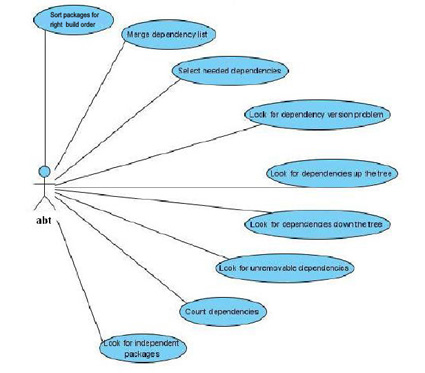
\includegraphics[bb=0 0 167 147]{ucd.jpg}
% ucd.jpg: 68.58dpi, width=6.19cm, height=5.44cm, bb=0 0 167 147
	\caption{User case diagram overview.}
	\label{fig:diagram}
\end{figure}

\newpage

\section{Use Case Survey}

\begin{figure}[htbp]
  \centering
  \includegraphics[angle=0,width=15cm,height=15cm]{"usecasediagram"}
  \caption{Use Case Diagram}
  \label{fig:ucdiagram}
\end{figure}

\subsection{Use Case Survey 1}

\begin{center}
\begin{tabularx}{\linewidth}{|l|p{7.08cm}|}
\hline
\textbf{Use Case Survey Name:} & Install Configuration\\
\hline
\textbf{Use Case Survey Number:} & 001 \\
\hline
\textbf{Initiating actor:} & AbT \\
\hline
\textbf{Description:} & A package containing a new configuration file will be installed. \\
\hline
\textbf{Completeness:} & Complete for Focused Stage \\
\hline
\textbf{Maturity:} & Mature for Focused Stage \\
\hline
\textbf{Dependency:} & None \\
\hline
\textbf{Source:} & Presentation by Eric Schabell \\
\hline
\end{tabularx}
\end{center}

\subsection{Use Case Survey 2}

\begin{center}
\begin{tabularx}{\linewidth}{|l|p{7.08cm}|}
\hline
\textbf{Use Case Survey Name:} & Upgrade Configuration \\
\hline
\textbf{Use Case Survey Number:} & 002 \\
\hline
\textbf{Initiating actor:} & AbT \\
\hline
\textbf{Description:} & Upgrade the current configuration to the new standard\\
\hline
\textbf{Completeness:} & Complete for Focused Stage \\
\hline
\textbf{Maturity:} & Mature for Focused Stage \\
\hline
\textbf{Dependency:} & None \\
\hline
\textbf{Source:} & Presentation by Eric Schabell \\
\hline
\end{tabularx}
\end{center}

\subsection{Use Case Survey 3}

\begin{center}
\begin{tabularx}{\linewidth}{|l|p{7.08cm}|}
\hline
\textbf{Use Case Survey Name:} & Backup Configuration \\
\hline
\textbf{Use Case Survey Number:} & 003 \\
\hline
\textbf{Initiating actor:} & AbT \\
\hline
\textbf{Description:} & Backup the current config file to a safe location \\
\hline
\textbf{Completeness:} & Complete for Focused Stage \\
\hline
\textbf{Maturity:} & Mature for Focused Stage \\
\hline
\textbf{Dependency:} & None \\
\hline
\textbf{Source:} & Presentation by Eric Schabell \\
\hline
\end{tabularx}
\end{center}

\subsection{Use Case Survey 4}

\begin{center}
\begin{tabularx}{\linewidth}{|l|p{7.08cm}|}
\hline
\textbf{Use Case Survey Name:} & Restore Configuration \\
\hline
\textbf{Use Case Survey Number:} & 004 \\
\hline
\textbf{Initiating actor:} & AbT \\
\hline
\textbf{Description:} & Restore a backup version of your configuration file \\
\hline
\textbf{Completeness:} & Complete for Focused Stage \\
\hline
\textbf{Maturity:} & Mature for Focused Stage \\
\hline
\textbf{Dependency:} & None \\
\hline
\textbf{Source:} & Presentation by Eric Schabell \\
\hline
\end{tabularx}
\end{center}

\subsection{Use Case Survey 5}

\begin{center}
\begin{tabularx}{\linewidth}{|l|p{7.08cm}|}
\hline
\textbf{Use Case Survey Name:} & Remove Configuration \\
\hline
\textbf{Use Case Survey Number:} & 005 \\
\hline
\textbf{Initiating actor:} & AbT \\
\hline
\textbf{Description:} & Delete a existing configuration from the system \\
\hline
\textbf{Completeness:} & Complete for Focused Stage \\
\hline
\textbf{Maturity:} & Mature for Focused Stage \\
\hline
\textbf{Dependency:} & None \\
\hline
\textbf{Source:} & Presentation by Eric Schabell \\
\hline
\end{tabularx}
\end{center}

\subsection{Use Case Survey 6}

\begin{center}
\begin{tabularx}{\linewidth}{|l|p{7.08cm}|}
\hline
\textbf{Use Case Survey Name:} & Edit Configuration \\
\hline
\textbf{Use Case Survey Number:} & 006 \\
\hline
\textbf{Initiating actor:} & AbT \\
\hline
\textbf{Description:} & Edit variables in a current configuration file \\
\hline
\textbf{Completeness:} & Complete for Focused Stage \\
\hline
\textbf{Maturity:} & Mature for Focused Stage \\
\hline
\textbf{Dependency:} & None \\
\hline
\textbf{Source:} & Presentation by Eric Schabell \\
\hline
\end{tabularx}
\end{center}

\subsection{Use Case Survey 7}

\begin{center}
\begin{tabularx}{\linewidth}{|l|p{7.08cm}|}
\hline
\textbf{Use Case Survey Name:} & Generate List of Configurations \\
\hline
\textbf{Use Case Survey Number:} & 007 \\
\hline
\textbf{Initiating actor:} & AbT \\
\hline
\textbf{Description:} & Generate a list containing every configuration file from the system \\
\hline
\textbf{Completeness:} & Complete for Focused Stage \\
\hline
\textbf{Maturity:} & Mature for Focused Stage \\
\hline
\textbf{Dependency:} & None \\
\hline
\textbf{Source:} & Presentation by Eric Schabell \\
\hline
\end{tabularx}
\end{center}

\subsection{Use Case Survey 8}

\begin{center}
\begin{tabularx}{\linewidth}{|l|p{7.08cm}|}
\hline
\textbf{Use Case Survey Name:} & Find Configuration \\
\hline
\textbf{Use Case Survey Number:} & 008 \\
\hline
\textbf{Initiating actor:} & AbT \\
\hline
\textbf{Description:} & Search the entire system for a configuration file identified by identifiers given by AbT \\
\hline
\textbf{Completeness:} & Complete for Focused Stage \\
\hline
\textbf{Maturity:} & Mature for Focused Stage \\
\hline
\textbf{Dependency:} & None \\
\hline
\textbf{Source:} & Discovered from a feedback session with Eric Schabell \\
\hline
\end{tabularx}
\end{center}

\section{Use Cases}
The requirements for this project are to be defined though \emph{Use Cases}
and are the basis for an initial 1.0 release. I wish for the final set of
requirements to be those needed to define a basic framework to manage the
software on a Linux machine. I consider these to provide that basic
functionality:

\subsection{General}
This section details items that are global in nature the \emph{AbTLinux}:

\begin{itemize}
\item source-based distro, binary as a bonus.
\item provide configuration file tools (view, edit, diff for smooth package updates).
\item suggest to install package if not installed and a command is entered from that package.
\item the abt package manager will be a command line interface.
\end{itemize}


\subsection{Packages}
This section details the requirements related to the packages themselves:

\begin{itemize}
\item install package
 
	\begin{itemize}
			\item if new install, just do it and generate logs.
			\item if upgrade, install over, compare old/new logs to delete what is not new.
	\end{itemize}

\item reinstall a package, either from cached build or rebuild/reconfigure.
\item remove package (includes check for lone package dependencies, ask user if wants to remove them)
\item downgrade a package to previous version
\item freeze a package in its current state (version holding)
\end{itemize}

%
% Use Cases - Packages.
%
\subsubsection{Install package}

\begin{tabularx}{\linewidth}{|l|X|}
\hline
\textbf{Use Case Name:} & \textbf{Install package} \\
\hline
\textbf{Description:} & 
The basic steps to be taken to install a software package. \\
\hline
\textbf{Actors:} & User \\
\hline
\textbf{Preconditions:} & Package description is available. \\
\hline
\textbf{Triggers:} & abt install $<$pkg$>$ \\
\hline
\textbf{Basic Course of Events:} & 
\begin{minipage}{\linewidth} 
  \vspace{0.05em}
  \begin{enumerate}
    \item User submits an install package request.
    \item Package to be installed is placed in install queue.
    \item \emph{Details} section of package is processed.
    \item \emph{Pre} section of package is processed.
    \item \emph{Configure} section of package is processed.
    \item Copy of configuration is saved.
    \item \emph{Build} section of package is processed.
    \item Copy of build is saved.
    \item \emph{Preinstall} section of package is processed.
    \item \emph{Install} section of package is processed.
    \item A list of installed files is saved.
    \item An integrity check is created on each installed file and saved.
    \item \emph{Post} section of package is processed.
    \item Package is added to installed packages list.
    \item Package is removed from install queue.
    \item Package build is cached for future usage.
    \item Package sources (build directories) are cleaned up (removed).
    \item User is notified that package was successfully installed.
  \end{enumerate}
  \vspace{0.05em}
\end{minipage}
\\
\hline
\end{tabularx}

\newpage
\begin{tabularx}{\linewidth}{|l|X|}
\hline
\textbf{Exceptions:} & 
\begin{minipage}{\linewidth} 
  \vspace{0.05em}
  \begin{enumerate}
    \item The package is already installed, report this and terminate with success.
    \item The \emph{details/pre/prebuild/preinstall/post} sections fail, report error and process stops.
    \item \emph{Configure} section fails, report error, save copy of configuration and process stops.
    \item \emph{Build} section fails, report error, save copy of build log and process stops.
    \item \emph{Install} section fails, report error, clean up any installed files (all or nothing is installed) and process stops.
    \item Dependency breakage detected, add broken package to install queue.
    \item Existing configuration files detected during installation of new files, query user to either; backup old versions and replace with new, keep old in place and copy new one next to it, replace old with new, default to the first choice.
  \end{enumerate}
  \vspace{0.05em}
\end{minipage}
\\
\hline 
\textbf{Postconditions:} &
\begin{minipage}{\linewidth}
  \vspace{0.05em}
  \begin{enumerate}
    \item Package is installed.
    \item For existing packages, when error is reported, then package is still in install queue.
    \item For broken dependencies, package added to install queue.
  \end{enumerate}
  \vspace{0.05em}
\end{minipage}
\\
\hline
\end{tabularx}




\newpage
\subsubsection{Reinstall package}
\begin{tabularx}{\linewidth}{|l|X|}
\hline
\textbf{Use Case Name:} & \textbf{Reinstall package} \\
\hline
\textbf{Description:} & 
The basic steps to be taken to reinstall (from cache or rebuild) a software package.\\
\hline
\textbf{Actors:} & User \\
\hline
\textbf{Preconditions:} & Package description is available and installed on system. \\
\hline
\textbf{Triggers:} & abt reinstall $<$pkg$>$ \\
\hline
\textbf{Basic Course of Events:} & 
\begin{minipage}{\linewidth} 
  \vspace{0.02em}
  \begin{enumerate}
    \item User submits a reinstall package request.
    \item User asked, install cached version or rebuild package.
    \item Rebuild requested, add to install queue.
    \item Previous configuration details available, query for reconfigure.
    \item \emph{Details} section of package is processed.
    \item \emph{Pre} section processed, reconfigure only if requested.
    \item \emph{Configure} section of package processed.
    \item Copy configuration created in temporary file.
    \item \emph{Prebuild} section of package processed.
    \item \emph{Build} section of package is processed.
    \item Copy of build created in temporary file.
    \item \emph{Preinstall} section of package processed.
    \item \emph{Install} section of package is processed.
    \item Installed files listed in temporary file.
    \item Create integrity check temp file on each installed file.
    \item \emph{Post} section of package is processed.
    \item Temporary files replace originals.
    \item Package listing in installed packages list updated.
    \item Package removed from install queue.
    \item Package sources removed.
    \item User notified package reinstalled.
  \end{enumerate}
  \vspace{0.02em}
\end{minipage}
\\
\hline
\end{tabularx}

\newpage
\begin{tabularx}{\linewidth}{|l|X|}
\hline
\textbf{Exceptions:} & 
\begin{minipage}{\linewidth} 
  \vspace{0.05em}
  \begin{enumerate}
    \item Any failures will result in created files (configuration and/or build) being saved with timestamp in file name.
    \item Any previous timestamped (unsuccessful reinstalls) will be removed, but original successful installs will remain.
    \item Any failures will result in user being given an error message with failure location information.
		\item Dependency breakage detected, add broken package to install queue.
    \item Existing configuration files detected during installation of new files, query user to either; backup old versions and replace with new, keep old in place and copy new one next to it, replace old with new, default to the first choice.
  \end{enumerate}
  \vspace{0.05em}
\end{minipage}
\\
\hline 
\textbf{Postconditions:} &
\begin{minipage}{\linewidth}
  \vspace{0.05em}
  \begin{enumerate}
    \item Package is reinstalled from cached version or rebuilt.
    \item New reinstall configuration, build, install and integrity files replace original installed files.
    \item For rebuild reinstalls (not for cached reinstalls) that fail, the package remains in the install queue.
		\item For broken dependencies, package added to install queue.
  \end{enumerate}
  \vspace{0.05em}
\end{minipage}
\\
\hline
\end{tabularx}




\newpage
\subsubsection{Remove package}

\begin{tabularx}{\linewidth}{|l|X|}
\hline
\textbf{Use Case Name:} & \textbf{Remove package} \\
\hline
\textbf{Description:} & 
Remove an installed package. \\
\hline
\textbf{Actors:} & User \\
\hline
\textbf{Preconditions:} & 
Requested package is installed. \\
\hline
\textbf{Triggers:} & abt remove $<$pkg$>$ \\
\hline
\textbf{Basic Course of Events:} & 
\begin{minipage}{\linewidth} 
  \vspace{0.05em}
  \begin{enumerate}
    \item User submits a remove package request.
    \item Check for dependency breakage, report for user input.
    \item Package is added to uninstall queue.
    \item Tarball is created containing the following:
    \begin{enumerate}
      \item Copy of installed configuration files.
      \item Copy of configuration.
      \item Copy of build.
      \item List of installed files.
      \item List of integrity checks for installed files.
      \item Copy of installed files.
      \item Copy of source files for this version.
      \item Copy of package data (detail, pre, configure, etc).
    \end{enumerate}
    \item Installed package files are removed.
    \item Package is removed from installed packages list.
    \item Package is removed from uninstall queue.
    \item Check for dependency breakage.
    \item User is notified that package was successfully uninstalled.
  \end{enumerate}
  \vspace{0.05em}
\end{minipage}
\\
\hline 
\textbf{Exceptions:} & 
If package not installed, exit with success.
\\
\hline 
\textbf{Postconditions:} &
\begin{minipage}{\linewidth}
  \vspace{0.05em}
  \begin{enumerate}
    \item The package is no longer installed.
    \item There is a tarball containing everything needed to re-create the package that was just removed.
    \item For broken dependencies, package added to install or uninstall queues.
  \end{enumerate}
  \vspace{0.05em}
\end{minipage}
\\
\hline
\end{tabularx}



\newpage
\subsubsection{Downgrade package}

\begin{tabularx}{\linewidth}{|l|X|}
\hline
\textbf{Use Case Name:} & \textbf{Downgrade a package} \\
\hline
\textbf{Description:} & 
Downgrade an installed package to a previously built version. \\
\hline
\textbf{Actors:} & User \\
\hline
\textbf{Preconditions:} & Previously requested version must be available. \\
\hline
\textbf{Triggers:} & abt downgrade $<$pkg$>$ $[$version$]$ \\
\hline
\textbf{Basic Course of Events:} & 
\begin{minipage}{\linewidth} 
  \vspace{0.05em}
  \begin{enumerate}
    \item User submits a request to downgrade a package.
    \item Check for dependency breakage, report for user input.
    \item If User requests specific version and it is available we run \emph{reinstall use case} for the cached version.
    \item if no version selected or version not available, User presented with a list of previously cached versions.
    \item User selects version to install.
    \item Using package versions tarball (contains all data saved on \emph{remove package use case}), User is led through the \emph{reinstall package use case}.
    \item Check for dependency breakage.
    \item User is notified that package was successfully downgraded to selected version.
  \end{enumerate}
  \vspace{0.05em}
\end{minipage}
\\
\hline 
\textbf{Exceptions:} & 
Requested versions are not available (empty list of cached versions), exit with error message.
\\
\hline 
\textbf{Postconditions:} &
\begin{minipage}{\linewidth}
  \vspace{0.05em}
  \begin{enumerate}
    \item Requested package version has been installed, downgrading installed package version.
    \item For broken dependencies, package added to install or uninstall queues.
  \end{enumerate}
  \vspace{0.05em}
\end{minipage}
\\
\hline
\end{tabularx}




\newpage
\subsubsection{Freeze package}

\begin{tabularx}{\linewidth}{|l|X|}
\hline
\textbf{Use Case Name:} & \textbf{Freeze a package} \\
\hline
\textbf{Description:} & 
Freeze a package at the currently installed version to prevent updates. \\
\hline
\textbf{Actors:} & User \\
\hline
\textbf{Preconditions:} & Package must be installed. \\
\hline
\textbf{Triggers:} & abt freeze $<$package$>$ \\
\hline
\textbf{Basic Course of Events:} & 
\begin{minipage}{\linewidth} 
  \vspace{0.05em}
  \begin{enumerate}
    \item User requests a package be frozen at current version number.
    \item User given chance to add a text note to frozen status.
    \item Package install list is annotated to show frozen status.
    \item User is notified that package has been frozen.
  \end{enumerate}
  \vspace{0.05em}
\end{minipage}
\\
\hline 
\textbf{Exceptions:} & 
\begin{minipage}{\linewidth} 
  \vspace{0.05em}
  \begin{enumerate}
    \item If package not installed then offer to install and freeze package.
    \item If package already has status frozen, complete process as if reset to frozen.
  \end{enumerate}
  \vspace{0.05em}
\end{minipage}
\\
\hline 
\textbf{Postconditions:} &
\begin{minipage}{\linewidth}
  \vspace{0.05em}
  \begin{enumerate}
    \item Package has been marked with status frozen.
    \item Package will not be queried for possible upgrade (version increase)
  \end{enumerate}
  \vspace{0.05em}
\end{minipage}
\\
\hline
\end{tabularx}





\newpage
\subsection{Queries}
This section details items related to queries a user / administrator would need to be
able to make on \emph{AbTLinux} machines:

\begin{itemize}
  \item show package details
  \item show installed packages
  \item show package install
  \item show package build
  \item show frozen packages
  \item show package dependencies
  \item show untracked files on system
  \item show journal
  \item show package that a file comes from
  \item search package description
  \item show install queue (all builds will be via a queue)
  \item show available update patch list (before retrieving them)
\end{itemize}

% 
% Use Cases - Queries.
%
\subsubsection{Show package details}

\begin{tabularx}{\linewidth}{|l|X|}
\hline
\textbf{Use Case Name:} & \textbf{Show package details} \\
\hline
\textbf{Description:} & Display the given packages details. \\
\hline
\textbf{Actors:} & User \\
\hline
\textbf{Preconditions:} & Package tree is available. \\
\hline
\textbf{Triggers:} & abt show-details $<$pkg$>$ \\
\hline
\textbf{Basic Course of Events:} & 
\begin{minipage}{\linewidth} 
  \vspace{0.05em}
  \begin{enumerate}
    \item User requests a show package.
    \item Package details displayed:
      \begin{enumerate}
        \item name
        \item version
        \item author
        \item source location
        \item last package update
        \item depencencies
        \item description
        \item installed version
        \item available version (from abt repository)
      \end{enumerate}
  \end{enumerate}
  \vspace{0.05em}
\end{minipage}
\\
\hline 
\textbf{Exceptions:} & none. \\
\hline 
\textbf{Postconditions:} &
User has seen the given packages details. \\
\hline
\end{tabularx}




%\newpage
\subsubsection{Show installed packages}

\begin{tabularx}{\linewidth}{|l|X|}
\hline
\textbf{Use Case Name:} & \textbf{Show installed packages} \\
\hline
\textbf{Description:} & Display a formatted listing of the installed packages. \\
\hline
\textbf{Actors:} & User \\
\hline
\textbf{Preconditions:} & Package install listing and network is available. \\
\hline
\textbf{Triggers:} & abt show-installed \\
\hline
\textbf{Basic Course of Events:} & 
\begin{minipage}{\linewidth} 
  \vspace{0.05em}
  \begin{enumerate}
    \item User requests an installed packages report.
    \item Access the installed packages listing.
    \item Access the remote update listing for most recent package versions.
    \item List presented containing the installed package details:
      \begin{enumerate}
        \item name
        \item date
        \item installed version
        \item available version local
        \item available version abt repository
      \end{enumerate}
  \end{enumerate}
  \vspace{0.05em}
\end{minipage}
\\
\hline 
\textbf{Exceptions:} & 
Remote package update listing is not available, complete report by filling in nothing for available version. \\
\hline 
\textbf{Postconditions:} &
User has been presented an overview of the installed packages. \\
\hline
\end{tabularx}



%\newpage
\subsubsection{Show package install}

\begin{tabularx}{\linewidth}{|l|X|}
\hline
\textbf{Use Case Name:} & \textbf{Show package install} \\
\hline
\textbf{Description:} & Display a listing of the files installed for given package. \\
\hline
\textbf{Actors:} & User \\
\hline
\textbf{Preconditions:} & Package requested is installed. \\
\hline
\textbf{Triggers:} & abt show-files $<$pkg$>$ \\
\hline
\textbf{Basic Course of Events:} & 
\begin{minipage}{\linewidth} 
  \vspace{0.05em}
  \begin{enumerate}
    \item User requests to view a listing of the files installed by a package.
    \item A dump is given of the installed files log for the package.
  \end{enumerate}
  \vspace{0.05em}
\end{minipage}
\\
\hline 
\textbf{Exceptions:} & Missing file log, report error. \\
\hline 
\textbf{Postconditions:} &
User has been presented a listing of the files installed by a package. \\
\hline
\end{tabularx}




%\newpage
\subsubsection{Show package build}

\begin{tabularx}{\linewidth}{|l|X|}
\hline
\textbf{Use Case Name:} & \textbf{Show package build} \\
\hline
\textbf{Description:} & Display the build log for given package. \\
\hline
\textbf{Actors:} & User \\
\hline
\textbf{Preconditions:} & Package requested has been built previously. \\
\hline
\textbf{Triggers:} & abt show-build $<$pkg$>$ \\
\hline
\textbf{Basic Course of Events:} & 
\begin{minipage}{\linewidth} 
  \vspace{0.05em}
  \begin{enumerate}
    \item User requests to view the most recent build log for package.
    \item A dump is given of the most recent build log for the package.
  \end{enumerate}
  \vspace{0.05em}
\end{minipage}
\\
\hline 
\textbf{Exceptions:} & Missing build log, report error. \\
\hline 
\textbf{Postconditions:} &
User has been presented a log of the given packages build. \\
\hline
\end{tabularx}




%\newpage
\subsubsection{Show frozen packages}

\begin{tabularx}{\linewidth}{|l|X|}
\hline
\textbf{Use Case Name:} & \textbf{Show frozen packages} \\
\hline
\textbf{Description:} & Display all packages with a frozen status. \\
\hline
\textbf{Actors:} & User \\
\hline
\textbf{Preconditions:} & none. \\
\hline
\textbf{Triggers:} & abt show-frozen \\
\hline
\textbf{Basic Course of Events:} & 
\begin{minipage}{\linewidth} 
  \vspace{0.05em}
  \begin{enumerate}
    \item User requests a list of frozen packages.
    \item The installed package list is used to determine which packages need to be checked.
    \item Packages that are determined to be frozen are displayed.
  \end{enumerate}
  \vspace{0.05em}
\end{minipage}
\\
\hline 
\textbf{Exceptions:} & Missing install log, report error. \\
\hline 
\textbf{Postconditions:} &
User has been presented a list of frozen packages. \\
\hline
\end{tabularx}




%\newpage
\subsubsection{Show packages dependencies}

\begin{tabularx}{\linewidth}{|l|X|}
\hline
\textbf{Use Case Name:} & \textbf{Show package dependencies} \\
\hline
\textbf{Description:} & Display the dependency tree for a given package. \\
\hline
\textbf{Actors:} & User \\
\hline
\textbf{Preconditions:} & none. \\
\hline
\textbf{Triggers:} & abt show-depends $<$pkg$>$ \\
\hline
\textbf{Basic Course of Events:} & 
\begin{minipage}{\linewidth} 
  \vspace{0.05em}
  \begin{enumerate}
    \item User requests to view dependencies for package.
    \item The dependency engine is used to generate a dependency tree (entire tree).
    \item The dependency tree is displayed for user to browse (both up and down the tree).
  \end{enumerate}
  \vspace{0.05em}
\end{minipage}
\\
\hline 
\textbf{Exceptions:} & none. \\
\hline 
\textbf{Postconditions:} &
User has been presented a dependency tree of the given package. \\
\hline
\end{tabularx}




%\newpage
\subsubsection{Show untracked files}

\begin{tabularx}{\linewidth}{|l|X|}
\hline
\textbf{Use Case Name:} & \textbf{Show untracked files} \\
\hline
\textbf{Description:} & Finds and displays a list of files not being tracked by abt. \\
\hline
\textbf{Actors:} & User \\
\hline
\textbf{Preconditions:} & none. \\
\hline
\textbf{Triggers:} & abt show-untracked \\
\hline
\textbf{Basic Course of Events:} & 
\begin{minipage}{\linewidth} 
  \vspace{0.05em}
  \begin{enumerate}
    \item User requests to view a list of untracked files.
    \item Using install logs as cross reference, list of untracked files is created.
    \item Display list of untracked files.
  \end{enumerate}
  \vspace{0.05em}
\end{minipage}
\\
\hline 
\textbf{Exceptions:} & Missing installed packages or install log files, report error. \\
\hline 
\textbf{Postconditions:} &
User has been presented a list of untracked files on the system. \\
\hline
\end{tabularx}




%\newpage
\subsubsection{Show journal}

\begin{tabularx}{\linewidth}{|l|X|}
\hline
\textbf{Use Case Name:} & \textbf{Show journal} \\
\hline
\textbf{Description:} & Display abt journal. \\
\hline
\textbf{Actors:} & User \\
\hline
\textbf{Preconditions:} & Abt journal exists. \\
\hline
\textbf{Triggers:} & abt show-journal \\
\hline
\textbf{Basic Course of Events:} & 
\begin{minipage}{\linewidth} 
  \vspace{0.05em}
  \begin{enumerate}
    \item User requests to view the abt journal.
    \item The abt journal is displayed.
  \end{enumerate}
  \vspace{0.05em}
\end{minipage}
\\
\hline 
\textbf{Exceptions:} & Missing journal, report error. \\
\hline 
\textbf{Postconditions:} &
User has been presented the journal. \\
\hline
\end{tabularx}




%\newpage
\subsubsection{Show file owner}

\begin{tabularx}{\linewidth}{|l|X|}
\hline
\textbf{Use Case Name:} & \textbf{Show file owner} \\
\hline
\textbf{Description:} & Display the owning package for a given file. \\
\hline
\textbf{Actors:} & User \\
\hline
\textbf{Preconditions:} & Package owning file is installed correctly. \\
\hline
\textbf{Triggers:} & abt show-owner $<$file$>$ \\
\hline
\textbf{Basic Course of Events:} & 
\begin{minipage}{\linewidth} 
  \vspace{0.05em}
  \begin{enumerate}
    \item User requests to view the owning package for a given file.
    \item The file may given as relative path or complete path.
    \item The install logs are searched to determine which package is owner.
    \item Owning package is displayed to user.
  \end{enumerate}
  \vspace{0.05em}
\end{minipage}
\\
\hline 
\textbf{Exceptions:} & File not found to be owned by a tracked package, show warning. \\
\hline 
\textbf{Postconditions:} &
User has been presented the name of the owning package for given file. \\
\hline
\end{tabularx}




%\newpage
\subsubsection{Search package descriptions}

\begin{tabularx}{\linewidth}{|l|X|}
\hline
\textbf{Use Case Name:} & \textbf{Search package descriptions} \\
\hline
\textbf{Description:} & 
Search all package descriptions for the given string, return package names that match. \\
\hline
\textbf{Actors:} & User \\
\hline
\textbf{Preconditions:} & Search string is normal string or a regexp. \\
\hline
\textbf{Triggers:} & abt search $<$string or regexp$>$ \\
\hline
\textbf{Basic Course of Events:} & 
\begin{minipage}{\linewidth} 
  \vspace{0.05em}
  \begin{enumerate}
    \item User submits a search string.
    \item All package descriptions are searched for match to given string.
    \item Packages matching are displayed to user.
  \end{enumerate}
  \vspace{0.05em}
\end{minipage}
\\
\hline 
\textbf{Exceptions:} & No matching string found, return warning. \\
\hline 
\textbf{Postconditions:} &
User has been presented with a list of packages with string matches from their descriptions. \\
\hline
\end{tabularx}



%\newpage
\subsubsection{Show install queue}

\begin{tabularx}{\linewidth}{|l|X|}
\hline
\textbf{Use Case Name:} & \textbf{Show install queue} \\
\hline
\textbf{Description:} & Display the install queue contents. \\
\hline
\textbf{Actors:} & User \\
\hline
\textbf{Preconditions:} & none. \\
\hline
\textbf{Triggers:} & abt show-iqueue \\
\hline
\textbf{Basic Course of Events:} & 
\begin{minipage}{\linewidth} 
  \vspace{0.05em}
  \begin{enumerate}
    \item User requests to view the contents of the install queue.
    \item The contents of the install queue is displayed.
  \end{enumerate}
  \vspace{0.05em}
\end{minipage}
\\
\hline 
\textbf{Exceptions:} & Missing install queue, create install queue and report empty queue. \\
\hline 
\textbf{Postconditions:} &
User has been presented with the contents of the install queue. \\
\hline
\end{tabularx}




%\newpage
\subsubsection{Show available patches}

\begin{tabularx}{\linewidth}{|l|X|}
\hline
\textbf{Use Case Name:} & \textbf{Show available patches} \\
\hline
\textbf{Description:} & Display all available patches. \\
\hline
\textbf{Actors:} & User \\
\hline
\textbf{Preconditions:} & Network available. \\
\hline
\textbf{Triggers:} & abt show-patches \\
\hline
\textbf{Basic Course of Events:} & 
\begin{minipage}{\linewidth} 
  \vspace{0.05em}
  \begin{enumerate}
    \item User requests to view all available patches.
    \item The list of available patches is retrieved from network.
    \item List of available patches displayed.
  \end{enumerate}
  \vspace{0.05em}
\end{minipage}
\\
\hline 
\textbf{Exceptions:} & Retrieval of patch listing fails, report error. \\
\hline 
\textbf{Postconditions:} &
User has been presented a complete list of available patches. \\
\hline
\end{tabularx}




\newpage
\subsection{Generation}
This section details items that need to be generated from an installed
machine:

\begin{itemize}
  \item list of packages needing updates
  \item HTML listing of package listing on box
\end{itemize}

%
% Use Cases - Generation.
%
\subsubsection{List package updates}

\begin{tabularx}{\linewidth}{|l|X|}
\hline
\textbf{Use Case Name:} & \textbf{List package updates} \\
\hline
\textbf{Description:} & 
Generate a list of updates available for installed packages. \\
\hline
\textbf{Actors:} & User \\
\hline
\textbf{Preconditions:} & 
Package install list and list of available updates from network are available. \\
\hline
\textbf{Triggers:} & abt show-updates \\
\hline
\textbf{Basic Course of Events:} & 
\begin{minipage}{\linewidth} 
  \vspace{0.05em}
  \begin{enumerate}
    \item User submits an updates request.
    \item Package install list is processed to check each package for updates.
    \item Available updates retrieved from over network.
    \item User is notified by showing available updates for all installed packages.
  \end{enumerate}
  \vspace{0.05em}
\end{minipage}
\\
\hline
\textbf{Exceptions:} & 
Warning when available update is older than installed package version.
\\
\hline 
\textbf{Postconditions:} &
Package updates list has been generated.
\\
\hline
\end{tabularx}




%\newpage
\subsubsection{HTML package listing}

\begin{tabularx}{\linewidth}{|l|X|}
\hline
\textbf{Use Case Name:} & \textbf{HTML package listing} \\
\hline
\textbf{Description:} & 
Generate HTML formatted listing of installed packages. \\
\hline
\textbf{Actors:} & User \\
\hline
\textbf{Preconditions:} & 
Package install list is available. \\
\hline
\textbf{Triggers:} & abt html \\
\hline
\textbf{Basic Course of Events:} & 
\begin{minipage}{\linewidth} 
  \vspace{0.05em}
  \begin{enumerate}
    \item User submits a html request.
    \item Package install list is processed.
    \item HTML page is generated showing installed packages list.
    \item User is notified of HTML page location.
  \end{enumerate}
  \vspace{0.05em}
\end{minipage}
\\
\hline
\textbf{Exceptions:} & none. \\
\hline 
\textbf{Postconditions:} &
HTML page showing package list has been generated.
\\
\hline
\end{tabularx}





%\newpage
\subsection{Downloads}
This section details the items that involve downloading diverse components
for \emph{AbTLinux} machines:

\begin{itemize}
  \item pull package sources
  \item pull package tree
  \item pull patches 
  \item pull news feed 
  \end{itemize}

%
% Use Cases - Downloads.
%
\subsubsection{Pull package sources}

\begin{tabularx}{\linewidth}{|l|X|}
\hline
\textbf{Use Case Name:} & \textbf{Pull package sources} \\
\hline
\textbf{Description:} & 
Downloading the source tarball for a given package. \\
\hline
\textbf{Actors:} & User \\
\hline
\textbf{Preconditions:} & 
Package description and network are available. \\
\hline
\textbf{Triggers:} & abt download $<$pkg$>$  \\
\hline
\textbf{Basic Course of Events:} & 
\begin{minipage}{\linewidth} 
  \vspace{0.05em}
  \begin{enumerate}
    \item User requests for package source(s) to be downloaded.
    \item The source location is obtained from the package description.
    \item Support for http(s), (s)ftp, cvs and subversion.
    \item Source is downloaded and placed in download location.
  \end{enumerate}
  \vspace{0.05em}
\end{minipage}
\\
\hline
\textbf{Exceptions:} & 
Source location is unreachable or gives error, report error. \\
\hline 
\textbf{Postconditions:} &
Package source(s) have been downloaded.
\\
\hline
\end{tabularx}




%\newpage
\subsubsection{Pull package tree}

\begin{tabularx}{\linewidth}{|l|X|}
\hline
\textbf{Use Case Name:} & \textbf{Pull package tree} \\
\hline
\textbf{Description:} & 
Downloading a package tree, optionally by tree name. \\
\hline
\textbf{Actors:} & User \\
\hline
\textbf{Preconditions:} & 
Network is available. \\
\hline
\textbf{Triggers:} & abt update $[$name$]$  \\
\hline
\textbf{Basic Course of Events:} & 
\begin{minipage}{\linewidth} 
  \vspace{0.05em}
  \begin{enumerate}
    \item User requests for package tree to be downloaded.
    \item Optional name given, then look up the location in registered list (internal).
    \item Support for http(s), (s)ftp, cvs, subversion and tla repositories.
    \item Package tree is downloaded and installed.
  \end{enumerate}
  \vspace{0.05em}
\end{minipage}
\\
\hline
\textbf{Exceptions:} & 
Source location is unreachable or gives error, report error. \\
\hline 
\textbf{Postconditions:} &
Package tree has been downloaded and installed.
\\
\hline
\end{tabularx}




%\newpage
\subsubsection{Pull patches}

\begin{tabularx}{\linewidth}{|l|X|}
\hline
\textbf{Use Case Name:} & \textbf{Pull patches} \\
\hline
\textbf{Description:} & 
Downloading available patches, optionally by repository name. \\
\hline
\textbf{Actors:} & User \\
\hline
\textbf{Preconditions:} & 
Network is available. \\
\hline
\textbf{Triggers:} & abt patches $[$name$]$  \\
\hline
\textbf{Basic Course of Events:} & 
\begin{minipage}{\linewidth} 
  \vspace{0.05em}
  \begin{enumerate}
    \item User requests for patches to be downloaded.
    \item Optional name given, then look up the location in registered list (internal).
    \item Support for http(s), (s)ftp, cvs, subversion and tla repositories.
    \item Patches are downloaded and applied.
  \end{enumerate}
  \vspace{0.05em}
\end{minipage}
\\
\hline
\textbf{Exceptions:} & 
Source location is unreachable or gives error, report error. \\
\hline 
\textbf{Postconditions:} &
Patches have been downloaded and applied.
\\
\hline
\end{tabularx}




%\newpage
\subsubsection{Pull news feed}

\begin{tabularx}{\linewidth}{|l|X|}
\hline
\textbf{Use Case Name:} & \textbf{Pull news feed} \\
\hline
\textbf{Description:} & 
Downloading and view available news feed. \\
\hline
\textbf{Actors:} & User \\
\hline
\textbf{Preconditions:} & 
Network is available. \\
\hline
\textbf{Triggers:} & abt news  \\
\hline
\textbf{Basic Course of Events:} & 
\begin{minipage}{\linewidth} 
  \vspace{0.05em}
  \begin{enumerate}
    \item User requests abt news feed download.
    \item Retrieve abt news feed file.
    \item Save and display news feed.
  \end{enumerate}
  \vspace{0.05em}
\end{minipage}
\\
\hline
\textbf{Exceptions:} & 
News feed location is unreachable or gives error, warning and attempt to display old news feed file. \\
\hline 
\textbf{Postconditions:} &
News feed has been downloaded and displayed.
\\
\hline
\end{tabularx}






\newpage
\subsection{Logging}
This section details the requirements for keeping track of work progress
with some form of logging. These items are the ones that require tracking:

\begin{itemize}
  \item log package installation, not tracking:

  \begin{itemize}
    \item /home
    \item /tmp
		\item /var/tmp
  \end{itemize}

  \item log package files integrity information (tool to use: md5)
  \item log package builds
  \item log general progression (journal)
  \item cached builds include all scripts needed to build so it can always be duplicated (not lost on package maintenance in the future), track the following for each package:

\begin{itemize}
  \item Major version number
  \item Build time (time installed package was built)
  \item Configuration time (time configuration last updated)
  \item Dependencies 
\end{itemize}

\end{itemize}

%
% Use Cases - Logging.
%
\subsubsection{Log package install}

\begin{tabularx}{\linewidth}{|l|X|}
\hline
\textbf{Use Case Name:} & \textbf{Log package install} \\
\hline
\textbf{Description:} & 
What will be logged from a package install. \\
\hline
\textbf{Actors:} & System \\
\hline
\textbf{Preconditions:} & none. \\
\hline
\textbf{Triggers:} & The install phase of a package install. \\
\hline
\textbf{Basic Course of Events:} & 
\begin{minipage}{\linewidth} 
  \vspace{0.05em}
  \begin{enumerate}
    \item A package will reach the \emph{Preinstall} section of package install.
    \item \emph{Install} section of package is processed.
    \item A list of installed files is logged.
    \item File in following directories are not tracked:
      \begin{enumerate}
        \item home directories.
        \item tmp directories.
        \item var/tmp directories.
      \end{enumerate}
  \end{enumerate}
  \vspace{0.05em}
\end{minipage}
\\
\hline
\textbf{Exceptions:} & 
Any failure to create log files will be reported as error. \\
\hline 
\textbf{Postconditions:} &
Package files installed have been tracked in log file. \\
\hline
\end{tabularx}




%\newpage
\subsubsection{Log package files integrity}

\begin{tabularx}{\linewidth}{|l|X|}
\hline
\textbf{Use Case Name:} & \textbf{Log package files integrity} \\
\hline
\textbf{Description:} & 
A log will be created with each file a package installs being integrity checked. \\
\hline
\textbf{Actors:} & System \\
\hline
\textbf{Preconditions:} & Integrity software is available on system. \\
\hline
\textbf{Triggers:} & The end of install phase of a package install. \\
\hline
\textbf{Basic Course of Events:} & 
\begin{minipage}{\linewidth} 
  \vspace{0.05em}
  \begin{enumerate}
    \item After files installed, the installed files log is parsed to create a checksum for each file.
    \item A file can be marked as a configuration file and not tracked.
    \item A file can be marked as shared and this will be noted in log.
    \item A log is created containing the resulting integrity information.
  \end{enumerate}
  \vspace{0.05em}
\end{minipage}
\\
\hline
\textbf{Exceptions:} & 
Any failure to create log files will be reported as error. \\
\hline 
\textbf{Postconditions:} &
Package files integrity information has been logged in a file. \\
\hline
\end{tabularx}




%\newpage
\subsubsection{Log package build}

\begin{tabularx}{\linewidth}{|l|X|}
\hline
\textbf{Use Case Name:} & \textbf{Log package build} \\
\hline
\textbf{Description:} & 
What will be logged from a package build. \\
\hline
\textbf{Actors:} & System \\
\hline
\textbf{Preconditions:} & none. \\
\hline
\textbf{Triggers:} & The build phase of a package install. \\
\hline
\textbf{Basic Course of Events:} & 
\begin{minipage}{\linewidth} 
  \vspace{0.05em}
  \begin{enumerate}
    \item \emph{Build} section of package is processed.
    \item The running of the package build is logged to a file.
  \end{enumerate}
  \vspace{0.05em}
\end{minipage}
\\
\hline
\textbf{Exceptions:} & 
Any failure to create log files will be reported as error. \\
\hline 
\textbf{Postconditions:} &
Package build has been logged in a file. \\
\hline
\end{tabularx}




%\newpage
\subsubsection{Log journal}

\begin{tabularx}{\linewidth}{|l|X|}
\hline
\textbf{Use Case Name:} & \textbf{Log journal} \\
\hline
\textbf{Description:} & 
Provide a journal of general abt activity. \\
\hline
\textbf{Actors:} & System \\
\hline
\textbf{Preconditions:} & none. \\
\hline
\textbf{Triggers:} & Any action abt does that is needing to be logged. \\
\hline
\textbf{Basic Course of Events:} & 
\begin{minipage}{\linewidth} 
  \vspace{0.05em}
  \begin{enumerate}
    \item Any item needing to be logged will be appended to the journal with timestamp.
    \item Auto journal rotation will be done at user defined number of lines or file size.
  \end{enumerate}
  \vspace{0.05em}
\end{minipage}
\\
\hline
\textbf{Exceptions:} & 
If activity journal does not exist, it will be created. \\
\hline 
\textbf{Postconditions:} &
Abt is able to log activity to the journal. \\
\hline
\end{tabularx}




%\newpage
\subsubsection{Log package cache}

\begin{tabularx}{\linewidth}{|l|X|}
\hline
\textbf{Use Case Name:} & \textbf{Log package cache} \\
\hline
\textbf{Description:} & 
A complete cache of a built package, including everything needed to duplicate 
the build at a later date. \\
\hline
\textbf{Actors:} & System \\
\hline
\textbf{Preconditions:} & none. \\
\hline
\textbf{Triggers:} & The end of a package install. \\
\hline
\textbf{Basic Course of Events:} & 
\begin{minipage}{\linewidth} 
  \vspace{0.05em}
  \begin{enumerate}
    \item At end of a complete package install a cache will be made, including:
    \item Copy of build configuration (preserve configuration time).
    \item Copy of build log (preserve build time).
    \item Copy of install log.
    \item Copy of package description (includes major version number).
    \item Copy of source.
    \item Copy of dependency tree.
  \end{enumerate}
  \vspace{0.05em}
\end{minipage}
\\
\hline
\textbf{Exceptions:} & 
Any failure to create cache will be reported as error. \\
\hline 
\textbf{Postconditions:} &
Package build has been cached. \\
\hline
\end{tabularx}






\newpage
\subsection{Fixing}
This section details requirements related to checking the health of
\emph{AbTLinux} machines and repairing any problems found:

\begin{itemize}
  \item remove unused package sources
  \item remove unused package logs
  \item verify installed package files
  \item verify installed package symlinks
  \item verify installed package dependencies (libraries, versions)
  \item verify system integrity 
  \item fix package(s)
\end{itemize}

%
% Use Cases - Fixing.
%
\subsubsection{Purge old package sources}

\begin{tabularx}{\linewidth}{|l|X|}
\hline
\textbf{Use Case Name:} & \textbf{Purge old package sources} \\
\hline
\textbf{Description:} & 
Source tarballs will be removed for packages that are no longer installed. 
This will remove source tarballs for any versions of installed packages other
than those currently installed. \\
\hline
\textbf{Actors:} & User \\
\hline
\textbf{Preconditions:} & Installed package list is available. \\
\hline
\textbf{Triggers:} & abt purge-src \\
\hline
\textbf{Basic Course of Events:} & 
\begin{minipage}{\linewidth} 
  \vspace{0.05em}
  \begin{enumerate}
    \item The user requests to remove unused package sources from system.
    \item The installed package list is used to determine which package (versions) to keep.
    \item All source tarballs from packages not currently installed are removed.
  \end{enumerate}
  \vspace{0.05em}
\end{minipage}
\\
\hline
\textbf{Exceptions:} & none. \\
\hline 
\textbf{Postconditions:} & All old source tarballs have been removed from the system. \\
\hline
\end{tabularx}




%\newpage
\subsubsection{Purge old logs}
\begin{tabularx}{\linewidth}{|l|X|}
\hline
\textbf{Use Case Name:} & \textbf{Purge old logs} \\
\hline
\textbf{Description:} & 
This command will query the user about removal of all old package logs (configuration, build,
install, integrity) and cache logs for packages that are no longer installed. \\
\hline
\textbf{Actors:} & User \\
\hline
\textbf{Preconditions:} & Installed package list is available. \\
\hline
\textbf{Triggers:} & abt purge-logs \\
\hline
\textbf{Basic Course of Events:} & 
\begin{minipage}{\linewidth} 
  \vspace{0.05em}
  \begin{enumerate}
    \item The user requests to remove old logs from the system.
    \item The user is queried whether cache logs also need to be removed.
    \item The installed package list is used to determine which package (versions) to keep.
    \item All package logs are removed from the system for packages not currently installed.
    \item Eventual cache logs are removed from the system for packages not currently installed.
  \end{enumerate}
  \vspace{0.05em}
\end{minipage}
\\
\hline
\textbf{Exceptions:} & none. \\
\hline 
\textbf{Postconditions:} & All old package log and eventual cache logs have been removed from the system. \\
\hline
\end{tabularx}




%\newpage
\subsubsection{Verify installed package files}

\begin{tabularx}{\linewidth}{|l|X|}
\hline
\textbf{Use Case Name:} & \textbf{Verify installed package files} \\
\hline
\textbf{Description:} & 
Verify that the given packages files are available on the system. 
\\
\hline
\textbf{Actors:} & User \\
\hline
\textbf{Preconditions:} & Package to be verified has a valid install log. \\
\hline
\textbf{Triggers:} & abt verify-files $<$pkg$>$ \\
\hline
\textbf{Basic Course of Events:} & 
\begin{minipage}{\linewidth} 
  \vspace{0.05em}
  \begin{enumerate}
    \item User submits a verify files request.
    \item Installed files for given package are checked if they exist by comparison to packages install log.
    \item After package checked, overview of eventual missing files reported to user.
  \end{enumerate}
  \vspace{0.05em}
\end{minipage}
\\
\hline 
\textbf{Exceptions:} & none. \\
\hline 
\textbf{Postconditions:} &
The installed files for given package have been verified, eventual missing files have been reported. \\
\hline
\end{tabularx}




%\newpage
\subsubsection{Verify installed package symlinks}

\begin{tabularx}{\linewidth}{|l|X|}
\hline
\textbf{Use Case Name:} & \textbf{Verify installed package symlinks} \\
\hline
\textbf{Description:} & 
Verify that the given packages symlinks are available on the system. 
\\
\hline
\textbf{Actors:} & User \\
\hline
\textbf{Preconditions:} & Package to be verified has a valid install log. \\
\hline
\textbf{Triggers:} & abt verify-symlinks $<$pkg$>$ \\
\hline
\textbf{Basic Course of Events:} & 
\begin{minipage}{\linewidth} 
  \vspace{0.05em}
  \begin{enumerate}
    \item User submits a verify symlinks request.
    \item Installed symlinks for given package are checked if they exist by comparison to packages install log.
    \item After package checked, overview of eventual missing symlinks reported to user.
  \end{enumerate}
  \vspace{0.05em}
\end{minipage}
\\
\hline 
\textbf{Exceptions:} & none. \\
\hline 
\textbf{Postconditions:} &
The installed symlinks for given package have been verified, eventual missing symlinks have been reported. \\
\hline
\end{tabularx}




%\newpage
\subsubsection{Verify installed package dependencies}

\begin{tabularx}{\linewidth}{|l|X|}
\hline
\textbf{Use Case Name:} & \textbf{Verify installed package deps} \\
\hline
\textbf{Description:} & 
Verify that the given packages dependencies are not broken (libraries).
\\
\hline
\textbf{Actors:} & User \\
\hline
\textbf{Preconditions:} & Package to be verified has a valid description. \\
\hline
\textbf{Triggers:} & abt verify-libs $<$pkg$>$ \\
\hline
\textbf{Basic Course of Events:} & 
\begin{minipage}{\linewidth} 
  \vspace{0.05em}
  \begin{enumerate}
    \item User submits a verify libraries request.
    \item Dependency engine used to determine given packages dependency tree.
    \item Installed files for each dependency are checked for existence.
    \item Installed symlinks for each dependency are checked for existence.
    \item After package checked, overview of eventual broken libraries reported to user.
  \end{enumerate}
  \vspace{0.05em}
\end{minipage}
\\
\hline 
\textbf{Exceptions:} & none. \\
\hline 
\textbf{Postconditions:} &
The installed libraries for given package have been verified, eventual discrepencies have been reported. \\
\hline
\end{tabularx}




%\newpage
\subsubsection{Verify installed package integrity}

\begin{tabularx}{\linewidth}{|l|X|}
\hline
\textbf{Use Case Name:} & \textbf{Verify installed package integrity} \\
\hline
\textbf{Description:} & 
Verify given packages files integrity.
\\
\hline
\textbf{Actors:} & User \\
\hline
\textbf{Preconditions:} & Package to be verified has a valid install log and md5 is available. \\
\hline
\textbf{Triggers:} & abt verify-integrity $<$pkg$>$ \\
\hline
\textbf{Basic Course of Events:} & 
\begin{minipage}{\linewidth} 
  \vspace{0.05em}
  \begin{enumerate}
    \item User submits a verify integrity request.
    \item Integrity of installed files for given package are checked by comparison to packages install log.
    \item After package checked, overview of eventual tainted files reported to user.
  \end{enumerate}
  \vspace{0.05em}
\end{minipage}
\\
\hline 
\textbf{Exceptions:} & none. \\
\hline 
\textbf{Postconditions:} &
The integrity of installed files for given package have been checked, eventual tainted files have been reported. \\
\hline
\end{tabularx}




%\newpage
\subsubsection{Fix package}

\begin{tabularx}{\linewidth}{|l|X|}
\hline
\textbf{Use Case Name:} & \textbf{Fix package} \\
\hline
\textbf{Description:} & 
Check the package for missing/broken libraries, symlinks and file permissions.
\\
\hline
\textbf{Actors:} & User \\
\hline
\textbf{Preconditions:} & Package to be fixed is installed. \\
\hline
\textbf{Triggers:} & abt fix $[$pkg$]$ \\
\hline
\textbf{Basic Course of Events:} & 
\begin{minipage}{\linewidth} 
  \vspace{0.05em}
  \begin{enumerate}
    \item User submits a fix request, either on a package or on entire installed packages list if no package is given.
    \item Package(s) are checked by comparing:
    \begin{enumerate}
      \item Installed files are checked if they exist.
      \item Installed files are checked for integrity.
      \item Installed libraries are checked for dependency breakage.
      \item Configuration files are checked only for existence.
    \end{enumerate}
    \item Any problems found result in User being asked if rebuild wanted.
    \item Default if User does not respond is to rebuild package.
    \item Check for possible dependency breakage.
    \item After package(s) checked, overview of good, bad and fixed package(s) reported to User.
  \end{enumerate}
  \vspace{0.05em}
\end{minipage}
\\
\hline 
\textbf{Exceptions:} & 
Any problems results in package(s) being left in the install or uninstall queues. 
\\
\hline 
\textbf{Postconditions:} &
\begin{minipage}{\linewidth}
  \vspace{0.05em}
  \begin{enumerate}
    \item User has report of good, bad and fixed package(s).
  \end{enumerate}
  \vspace{0.05em}
\end{minipage}
\\
\hline
\end{tabularx}






\newpage
\subsection{Patching}
This section details the requirements related to providing patching for
updates and fixes on \emph{AbTLinux} machines:

\begin{itemize}
  \item provide for updating with a patch per package
  \item provide package tree patches (i.e. for entire stable tree)
\end{itemize}

%
% Use Cases - Patching.
%
\subsubsection{Patch package update}

\begin{tabularx}{\linewidth}{|l|X|}
\hline
\textbf{Use Case Name:} & \textbf{Patch package update} \\
\hline
\textbf{Description:} & 
Patches will be provided as preferred method of updating a package, fall-back
is to use the complete updated package description. \\
\hline
\textbf{Actors:} & User \\
\hline
\textbf{Preconditions:} & 
Patch is available over the network and package is installed. \\
\hline
\textbf{Triggers:} & Any command leading to update or fix from AbTLinux network.  \\
\hline
\textbf{Basic Course of Events:} & 
\begin{minipage}{\linewidth} 
  \vspace{0.05em}
  \begin{enumerate}
    \item User request leading to an update or fix being needed over the network.
    \item Attempt is made to retrieve needed patch over network.
    \item Fall-back is to retrieve needed package (entire package description) over network.
    \item Package is updated with patch or new package description and left in install queue.
  \end{enumerate}
  \vspace{0.05em}
\end{minipage}
\\
\hline
\textbf{Exceptions:} & 
Patch fails to be applied, fall-back to entire package description update. \\
\hline 
\textbf{Postconditions:} &
Package has been updated with patch if available, otherwise with complete package listing.
\\
\hline
\end{tabularx}




%\newpage
\subsubsection{Patch package tree update}

\begin{tabularx}{\linewidth}{|l|X|}
\hline
\textbf{Use Case Name:} & \textbf{Patch package tree update} \\
\hline
\textbf{Description:} & 
Patches will be provided as preferred method of updating a package tree, fall-back
is to use the complete updated package tree. \\
\hline
\textbf{Actors:} & User \\
\hline
\textbf{Preconditions:} & 
Patch is available over the network. \\
\hline
\textbf{Triggers:} & Any command leading to update of the entire package tree from AbTLinux network.  \\
\hline
\textbf{Basic Course of Events:} & 
\begin{minipage}{\linewidth} 
  \vspace{0.05em}
  \begin{enumerate}
    \item User request leading to an update of the entire package tree over the network.
    \item Attempt is made to retrieve the tree patch over network.
    \item Fall-back is to retrieve entire tree over network.
    \item Package tree is updated with patch or entire new tree.
  \end{enumerate}
  \vspace{0.05em}
\end{minipage}
\\
\hline
\textbf{Exceptions:} & 
Patch fails to be applied, fall back to entire new tree. \\
\hline 
\textbf{Postconditions:} &
Package tree has been updated with patch if available, otherwise with complete new tree.
\\
\hline
\end{tabularx}






\newpage
\subsection{Maintaining}
This section details the requirements related to maintenance tasks on
\emph{AbTLinux} machines:

\begin{itemize}
  \item provide for central build box (clients pull package builds from central box)
  \item provide for specification of package sources download location
\end{itemize}

%
% Use Cases - Maintaining.
%
\subsubsection{Central build}

\begin{tabularx}{\linewidth}{|l|X|}
\hline
\textbf{Use Case Name:} & \textbf{Central build} \\
\hline
\textbf{Description:} & 
Allows a single machine to function as a build center, providing cached software package
builds for other machines on a network. \\
\hline
\textbf{Actors:} & User \\
\hline
\textbf{Preconditions:} & 
Network is available. \\
\hline
\textbf{Triggers:} & 
User setup is pointing to this central server as provider of cached software packages
and requests a package install or update. \\
\hline
\textbf{Basic Course of Events:} & 
\begin{minipage}{\linewidth} 
  \vspace{0.05em}
  \begin{enumerate}
    \item User request leading to an (re)-install, update or fix of package being needed.
    \item User setup to direct all request to remote machine for cached packages.
    \item Fall-back is to search for cached packages on local machine.
    \item Cached package is retrieved and installed on local machine.
    \item A fix package check is run.
    \item User notified that package installed successfully.
  \end{enumerate}
  \vspace{0.05em}
\end{minipage}
\\
\hline
\textbf{Exceptions:} & 
Unable to obtain cached package from central server, fall-back to local machine. \\
\hline 
\textbf{Postconditions:} &
Cached package has been installed and checked successfully. \\
\hline
\end{tabularx}




%\newpage
\subsubsection{Source location package tree}

\begin{tabularx}{\linewidth}{|l|X|}
\hline
\textbf{Use Case Name:} & \textbf{Source location package tree} \\
\hline
\textbf{Description:} & 
User can specify package tree repository, default being the AbTLinux provided repository. \\
\hline
\textbf{Actors:} & User \\
\hline
\textbf{Preconditions:} & 
Given repository is available and reachable. \\
\hline
\textbf{Triggers:} & 
User requests to set a package tree repository location. \\
\hline
\textbf{Basic Course of Events:} & 
\begin{minipage}{\linewidth} 
  \vspace{0.05em}
  \begin{enumerate}
    \item User provides a given URI as default package tree repository.
    \item Fall-back is to use the AbTLinux provided repository.
    \item User requests package tree update.
    \item Package tree is updated from given URI.
    \item User notified that package tree updated successfully.
  \end{enumerate}
  \vspace{0.05em}
\end{minipage}
\\
\hline
\textbf{Exceptions:} & 
Unable to obtain package tree from URI, fall-back to AbTLinux repository. \\
\hline 
\textbf{Postconditions:} &
Package tree has been updated successfully. \\
\hline
\end{tabularx}




\subsection{Dependencies}
This section will be covered in an apart requirements document, focusing on
the
entire dependency engine problem. This will be a student project for the course 
Requirements Engineering at the Radboud University Nijmegen. 

%This section details the requirements related to dependencies between
%packages and how to deal with them:

%\begin{itemize}
%    \item dependency will specify a version (or use default?)
%    \item dependency can be optional
%    \item dependencies will be ordered for a correct build process (dep engine!)
%    \item support build-time and run-time dependencies:

%    \begin{itemize}
%        \item RELIES ON (RO) - 'A' RO 'B'; then 'A' will be rebuilt anytime 'B' is rebuilt.
%        \item DEPENDS ON (DO) - 'A' DO 'B'; then 'A' will be rebuilt if 'B' config changes.
%				\item a buildDep is a dependency needed to build some package.
%        \item leads to several types of depends:

%        \begin{itemize}

%            \item permanently relies on
%            \item permanently depends on
%            \item optionally relies on
%            \item optionally depends on
%        \end{itemize}

%    \end{itemize}

%    \item prevent removal of packages with DEPENDS ON (DO) dependencies.
%    \item auto add packages with RELIES ON (RO) dependencies to build queue if user rebuilds a package that relies on it.

%\end{itemize}



\newpage
\section{Scenarios}  
Here I will work out the use scenarios into example scenarios filled with actual
data.


\subsection{Packages}
\medskip

\begin{tabularx}{\linewidth}{|l|X|}
\hline
\textbf{Use Case Name:} & \textbf{Install package} \\
\hline
\textbf{Use Case Steps:} & 
\begin{minipage}{\linewidth} 
  \vspace{0.05em}
  \begin{enumerate}
   \item Steps
  \end{enumerate}
  \vspace{0.05em}
\end{minipage}
\\
\hline 
\textbf{Alternative Path:} &
\begin{minipage}{\linewidth}
  \vspace{0.05em} 
  \begin{enumerate}
    \item Steps
  \end{enumerate}
  \vspace{0.05em} 
\end{minipage}
\\
\hline
\end{tabularx}

\newpage



\medskip

\begin{tabularx}{\linewidth}{|l|X|}
\hline
\textbf{Use Case Name:} & \textbf{Reinstall package} \\
\hline
\textbf{Use Case Steps:} & 
\begin{minipage}{\linewidth} 
  \vspace{0.05em}
  \begin{enumerate}
   \item Steps
  \end{enumerate}
  \vspace{0.05em}
\end{minipage}
\\
\hline 
\textbf{Alternative Path:} &
\begin{minipage}{\linewidth}
  \vspace{0.05em} 
  \begin{enumerate}
    \item Steps
  \end{enumerate}
  \vspace{0.05em} 
\end{minipage}
\\
\hline
\end{tabularx}

\newpage


\medskip

\begin{tabularx}{\linewidth}{|l|X|}
\hline
\textbf{Use Case Name:} & \textbf{Remove package} \\
\hline
\textbf{Use Case Steps:} & 
\begin{minipage}{\linewidth} 
  \vspace{0.05em}
  \begin{itemize}
    \item User command \textbf{'abt remove fortune'}.
    \item \textbf{fortune} added to remove queue.
    \item \emph{Details} section processed:
    \begin{enumerate}
      \item NAME = fortune
      \item VERSION = \url{mod-9708}
      \item SRCFILE = \url{fortune-mod-9708.tar.gz}
      \item SRCDIR = \url{/usr/src/fortune-mod-9708}
      \item SRCURL = \url{http://www.fortune.org/pub/fortune-mod-9708.tar.gz}
      \item INTEGRITY = c016e3549942cbb
      \item URL = \url{http://www.fortune.org}
      \item LICENSE = BSD
      \item DESCRIPTION = "Random quotations from a large database."
    \end{enumerate}
    \item Check to ensure package installed.
    \item Dependencies for this package are checked.
    \item Eventual broken dependencies are added to install queue to be rebuilt.
    \item Retrieve fortune logs: \url{/var/log/abt/*/fortune-mod-9708/*}.
    \begin{enumerate}
      \item Package configure file: \url{/var/log/abt/configure/}.
      \item Package build file: \url{/var/log/abt/build/}.
      \item Package install file: \url{/var/log/abt/install/}.
      \item Package integrity file: \url{/var/log/abt/integrity/}.
      \item Package sources: \url{/var/spool/abt/fortune-mod-9708.tar.gz}
    \end{enumerate}
    \item \emph{Preremove} section processed:
    \begin{enumerate}
      \item Process any given special instructions found here.
    \end{enumerate}
  \end{itemize}
  \vspace{0.05em}
\end{minipage}
\\
\hline 
\end{tabularx}

\begin{tabularx}{\linewidth}{|l|X|}
\hline
\textbf{Use Case Steps:} & 
\begin{minipage}{\linewidth} 
  \vspace{0.05em}
  \begin{itemize}
    \item Files cached in \url{/var/state/abt/cached/fortune/*}.
    \item Process any configuration files:
    \begin{enumerate}
      \item Cache copies of existing configuration files: \url{fortune_mod-9708.user-configs}.
      \item Base removal/keeping of existing configuration files on user provided option (globally set).
    \end{enumerate}
    \item Create compressed tarball of all relevant logs.
    \item Remove fortune installed files.
    \item User notified that fortune-mod-9708 has been successfully removed.
  \end{itemize}
  \vspace{0.05em}
\end{minipage}
\\
\hline 
\textbf{Alternative Path:} & None. \\
\hline
\end{tabularx}

\newpage



\medskip

\begin{tabularx}{\linewidth}{|l|X|}
\hline
\textbf{Use Case Name:} & \textbf{Downgrade package} \\
\hline
\textbf{Use Case Steps:} & 
\begin{minipage}{\linewidth} 
  \vspace{0.05em}
  \begin{itemize}
    \item User command \textbf{'abt downgrade fortune mod-9707'}.
    \item \textbf{fortune} added to install queue.
    \item Check to ensure \textbf{fortune} package installed and version higher, mod-9708.
    \item Dependencies for package are checked.
    \item Eventual broken dependencies are added to install queue to be rebuilt.
    \item Run \textit{remove package scenario} for fortune mod-9708.
    \item Retrieve cached data for fortune mod-9707:
    \begin{enumerate}
      \item \url{/var/state/abt/cached/fortune/*}.
    \end{enumerate}
    \item Unpack and reinstall the package following \textit{install package scenario}.
    \item User notified that fortune has been successfully downgraded.
  \end{itemize}
  \vspace{0.05em}
\end{minipage}
\\
\hline
\textbf{Alternative Path:} & None. 
\\
\hline
\end{tabularx}
\medskip

\begin{tabularx}{\linewidth}{|l|X|}
\hline
\textbf{Use Case Name:} & \textbf{Freeze package} \\
\hline
\textbf{Use Case Steps:} & 
\begin{minipage}{\linewidth} 
  \vspace{0.05em}
  \begin{itemize}
   \item User command \textbf{'abt freeze fortune'}.
    \item Check to ensure \textbf{fortune} package installed.
    \item Add \textbf{fortune} to the frozen packages list:
    \begin{enumerate}
      \item Save \url{/var/state/abt/frozen/fortune.frozen}.
      \item This file will include a date and any other relevant information.
    \end{enumerate}
    \item User notified that fortune has been successfully frozen.
  \end{itemize}
  \vspace{0.05em}
\end{minipage}
\\
\hline 
\textbf{Alternative Path:} & None. \\
\hline
\end{tabularx}


\subsection{Queries}
\medskip

\begin{tabularx}{\linewidth}{|l|X|}
\hline
\textbf{Use Case Name:} & \textbf{Show package details} \\
\hline
\textbf{Use Case Steps:} & 
\begin{minipage}{\linewidth} 
  \vspace{0.05em}
  \begin{itemize}
    \item User command \textbf{'abt show-details fortune'}.
    \item \emph{Details} section processed:
    \begin{enumerate}
      \item NAME = fortune
      \item VERSION = \url{mod-9708}
      \item SRCFILE = \url{fortune-mod-9708.tar.gz}
      \item SRCDIR = \url{/usr/src/fortune-mod-9708}
      \item SRCURL = \url{http://www.fortune.org/pub/fortune-mod-9708.tar.gz}
      \item INTEGRITY = c016e3549942cbb
      \item URL = \url{http://www.fortune.org}
      \item LICENSE = BSD
      \item DESCRIPTION = "Random quotations from a large database."
    \end{enumerate}
    \item This data displayed for the user.
  \end{itemize}
  \vspace{0.05em}
\end{minipage}
\\
\hline 
\textbf{Alternative Path:} &
\begin{minipage}{\linewidth}
  \vspace{0.05em} 
  \begin{enumerate}
    \item Requested package is unavailabel, user receives warning.
  \end{enumerate}
  \vspace{0.05em} 
\end{minipage}
\\
\hline
\end{tabularx}
\medskip

\begin{tabularx}{\linewidth}{|l|X|}
\hline
\textbf{Use Case Name:} & \textbf{Show installed packages} \\
\hline
\textbf{Use Case Steps:} & 
\begin{minipage}{\linewidth} 
  \vspace{0.05em}
  \begin{itemize}
    \item User command \textbf{'abt show-installed'}.
    \item Installed packages information is acquired from install info location.
    \item For each package that is installed the following is displayed:
    \begin{enumerate}
      \item package name
      \item package version
      \item package install date
      \item package version available (obtain from current package description).
    \end{enumerate}
  \end{itemize}
  \vspace{0.05em}
\end{minipage}
\\
\hline 
\textbf{Alternative Path:} &
\begin{minipage}{\linewidth}
  \vspace{0.05em} 
  \begin{enumerate}
    \item Unable to generate installed packages list, warn user.
  \end{enumerate}
  \vspace{0.05em} 
\end{minipage}
\\
\hline
\end{tabularx}
\medskip

\begin{tabularx}{\linewidth}{|l|X|}
\hline
\textbf{Use Case Name:} & \textbf{Show package install} \\
\hline
\textbf{Use Case Steps:} & 
\begin{minipage}{\linewidth} 
  \vspace{0.05em}
  \begin{itemize}
    \item User command \textbf{'abt show-files fortune'}.
    \item Installed files information for is acquired from fortune install log location.
    \item The install log is displayed for the user.
  \end{itemize}
  \vspace{0.05em}
\end{minipage}
\\
\hline 
\textbf{Alternative Path:} &
\begin{minipage}{\linewidth}
  \vspace{0.05em} 
  \begin{enumerate}
    \item Fortune install log is not available, warn user.
  \end{enumerate}
  \vspace{0.05em} 
\end{minipage}
\\
\hline
\end{tabularx}
\medskip

\begin{tabularx}{\linewidth}{|l|X|}
\hline
\textbf{Use Case Name:} & \textbf{Show package build} \\
\hline
\textbf{Use Case Steps:} & 
\begin{minipage}{\linewidth} 
  \vspace{0.05em}
  \begin{enumerate}
   \item Steps
  \end{enumerate}
  \vspace{0.05em}
\end{minipage}
\\
\hline 
\textbf{Alternative Path:} &
\begin{minipage}{\linewidth}
  \vspace{0.05em} 
  \begin{enumerate}
    \item Steps
  \end{enumerate}
  \vspace{0.05em} 
\end{minipage}
\\
\hline
\end{tabularx}

\newpage


\medskip

\begin{tabularx}{\linewidth}{|l|X|}
\hline
\textbf{Use Case Name:} & \textbf{Show frozen packages} \\
\hline
\textbf{Use Case Steps:} & 
\begin{minipage}{\linewidth} 
  \vspace{0.05em}
  \begin{itemize}
    \item User command \textbf{'abt show-frozen'}.
    \item List of frozen packages is acquired from frozen log location.
    \item The frozen packages are displayed for the user:
    \begin{enumerate}
      \item package name
      \item package version
      \item date frozen
    \end{enumerate}
  \end{itemize}
  \vspace{0.05em}
\end{minipage}
\\
\hline 
\textbf{Alternative Path:} &
\begin{minipage}{\linewidth}
  \vspace{0.05em} 
  \begin{enumerate}
    \item Frozen log is unavailable, warn user.
  \end{enumerate}
  \vspace{0.05em} 
\end{minipage}
\\
\hline
\end{tabularx}
\medskip

\begin{tabularx}{\linewidth}{|l|X|}
\hline
\textbf{Use Case Name:} & \textbf{Show package dependencies} \\
\hline
\textbf{Use Case Steps:} & 
\begin{minipage}{\linewidth} 
  \vspace{0.05em}
  \begin{itemize}
    \item User command \textbf{'abt show-depends fortune'}.
    \item The depEngine is queried for a list of dependencies from fortune:
    \begin{enumerate}
      \item all currently installed packages that DependsOn fortune.
      \item all currently installed packages that ReliesOn fortune.
      \item all currently installed packages that optionally DependsOn fortune.
      \item all currently installed packages that optionally ReliesOn fortune.
      \item same as previous items, but that fortune (optionally) DependsOn/ReliesOn.
    \end{enumerate}
    \item The list generated by the depEngine is displayed for the user:
    \begin{enumerate}
      \item name of package
      \item version of package
    \end{enumerate}
  \end{itemize}

  \vspace{0.05em}
\end{minipage}
\\
\hline 
\textbf{Alternative Path:} &
\begin{minipage}{\linewidth}
  \vspace{0.05em} 
  \begin{enumerate}
    \item DepEngine is unavailable, warn user.
    \item Returned list is empty of dependencies, warn user.
    \item Fortune is not installed, warn user.
  \end{enumerate}
  \vspace{0.05em} 
\end{minipage}
\\
\hline
\end{tabularx}
\medskip

\begin{tabularx}{\linewidth}{|l|X|}
\hline
\textbf{Use Case Name:} & \textbf{Show untracked files} \\
\hline
\textbf{Use Case Steps:} & 
\begin{minipage}{\linewidth} 
  \vspace{0.05em}
  \begin{enumerate}
   \item Steps
  \end{enumerate}
  \vspace{0.05em}
\end{minipage}
\\
\hline 
\textbf{Alternative Path:} &
\begin{minipage}{\linewidth}
  \vspace{0.05em} 
  \begin{enumerate}
    \item Steps
  \end{enumerate}
  \vspace{0.05em} 
\end{minipage}
\\
\hline
\end{tabularx}

\newpage


\medskip

\begin{tabularx}{\linewidth}{|l|X|}
\hline
\textbf{Use Case Name:} & \textbf{Show journal} \\
\hline
\textbf{Use Case Steps:} & 
\begin{minipage}{\linewidth} 
  \vspace{0.05em}
  \begin{enumerate}
   \item Steps
  \end{enumerate}
  \vspace{0.05em}
\end{minipage}
\\
\hline 
\textbf{Alternative Path:} &
\begin{minipage}{\linewidth}
  \vspace{0.05em} 
  \begin{enumerate}
    \item Steps
  \end{enumerate}
  \vspace{0.05em} 
\end{minipage}
\\
\hline
\end{tabularx}

\newpage


\medskip

\begin{tabularx}{\linewidth}{|l|X|}
\hline
\textbf{Use Case Name:} & \textbf{Show file owner} \\
\hline
\textbf{Use Case Steps:} & 
\begin{minipage}{\linewidth} 
  \vspace{0.05em}
  \begin{itemize}
    \item User command \textbf{'abt show-owner $<$file$>$'}.
    \item Install logs at \url{/var/state/abt/install/*.install} are checked for the file.
    \item Package name as file owner reported to user.
  \end{itemize}
  \vspace{0.05em}
\end{minipage}
\\
\hline 
\textbf{Alternative Path:} &
\begin{minipage}{\linewidth}
  \vspace{0.05em} 
  \begin{enumerate}
    \item File not found in install logs, report to user.
    \item File submitted was not full path can result in multiple package results.
  \end{enumerate}
  \vspace{0.05em} 
\end{minipage}
\\
\hline
\end{tabularx}
\medskip

\begin{tabularx}{\linewidth}{|l|X|}
\hline
\textbf{Use Case Name:} & \textbf{Search package descriptions} \\
\hline
\textbf{Use Case Steps:} & 
\begin{minipage}{\linewidth} 
  \vspace{0.05em}
  \begin{itemize}
    \item User command \textbf{'abt search <string/regexp>'}.
    \item Search all package descriptions for the given string/regexp.
    \item Report list of package names with descriptions that match the search string/regexp.
  \end{itemize}
  \vspace{0.05em}
\end{minipage}
\\
\hline 
\textbf{Alternative Path:} &
\begin{minipage}{\linewidth}
  \vspace{0.05em} 
  \begin{enumerate}
    \item No matches to string/regexp found, report to user.
    \item No package descriptions available, warn to user.
  \end{enumerate}
  \vspace{0.05em} 
\end{minipage}
\\
\hline
\end{tabularx}
\medskip

\begin{tabularx}{\linewidth}{|l|X|}
\hline
\textbf{Use Case Name:} & \textbf{Show install queue} \\
\hline
\textbf{Use Case Steps:} & 
\begin{minipage}{\linewidth} 
  \vspace{0.05em}
  \begin{itemize}
    \item User command \textbf{'abt show-iqueue'}.
    \item Display the contents of the install queue.
  \end{itemize}
  \vspace{0.05em}
\end{minipage}
\\
\hline 
\textbf{Alternative Path:} &
\begin{minipage}{\linewidth}
  \vspace{0.05em} 
  \begin{enumerate}
    \item Install queue file is non-existent or empty, report to user.
  \end{enumerate}
  \vspace{0.05em} 
\end{minipage}
\\
\hline
\end{tabularx}
\medskip

\begin{tabularx}{\linewidth}{|l|X|}
\hline
\textbf{Use Case Name:} & \textbf{Show available patches} \\
\hline
\textbf{Use Case Steps:} & 
\begin{minipage}{\linewidth} 
  \vspace{0.05em}
  \begin{enumerate}
   \item Steps
  \end{enumerate}
  \vspace{0.05em}
\end{minipage}
\\
\hline 
\textbf{Alternative Path:} &
\begin{minipage}{\linewidth}
  \vspace{0.05em} 
  \begin{enumerate}
    \item Steps
  \end{enumerate}
  \vspace{0.05em} 
\end{minipage}
\\
\hline
\end{tabularx}

\newpage




\subsection{Generation}
\medskip

\begin{tabularx}{\linewidth}{|l|X|}
\hline
\textbf{Use Case Name:} & \textbf{List package updates} \\
\hline
\textbf{Use Case Steps:} & 
\begin{minipage}{\linewidth} 
  \vspace{0.05em}
  \begin{enumerate}
   \item Steps
  \end{enumerate}
  \vspace{0.05em}
\end{minipage}
\\
\hline 
\textbf{Alternative Path:} &
\begin{minipage}{\linewidth}
  \vspace{0.05em} 
  \begin{enumerate}
    \item Steps
  \end{enumerate}
  \vspace{0.05em} 
\end{minipage}
\\
\hline
\end{tabularx}

\newpage



\medskip

\begin{tabularx}{\linewidth}{|l|X|}
\hline
\textbf{Use Case Name:} & \textbf{HTML package listing} \\
\hline
\textbf{Use Case Steps:} & 
\begin{minipage}{\linewidth} 
  \vspace{0.05em}
  \begin{itemize}
    \item User command \textbf{'abt html'}.
    \item Generate HTML page from installed packages listing; \textbf{package name with hyperlink to website, version installed.}
  \end{itemize}
  \vspace{0.05em}
\end{minipage}
\\
\hline 
\textbf{Alternative Path:} &
\begin{minipage}{\linewidth}
  \vspace{0.05em} 
  \begin{enumerate}
    \item Installed package listing unavailable, warn user.
  \end{enumerate}
  \vspace{0.05em} 
\end{minipage}
\\
\hline
\end{tabularx}


\subsection{Downloads}
\medskip

\begin{tabularx}{\linewidth}{|l|X|}
\hline
\textbf{Use Case Name:} & \textbf{Pull package sources} \\
\hline
\textbf{Use Case Steps:} & 
\begin{minipage}{\linewidth} 
  \vspace{0.05em}
  \begin{enumerate}
   \item Steps
  \end{enumerate}
  \vspace{0.05em}
\end{minipage}
\\
\hline 
\textbf{Alternative Path:} &
\begin{minipage}{\linewidth}
  \vspace{0.05em} 
  \begin{enumerate}
    \item Steps
  \end{enumerate}
  \vspace{0.05em} 
\end{minipage}
\\
\hline
\end{tabularx}

\newpage



\medskip

\begin{tabularx}{\linewidth}{|l|X|}
\hline
\textbf{Use Case Name:} & \textbf{Pull package tree} \\
\hline
\textbf{Use Case Steps:} & 
\begin{minipage}{\linewidth} 
  \vspace{0.05em}
  \begin{itemize}
    \item User command \textbf{'abt update $<$name$>$'}.
    \item If name is given, then update only that package tree via the source location entry.
    \item Otherwise update all registered package trees.
    \item Package tree(s) updated, \textbf{'svn -r REPO-NAME update'}.
    \item Report to user update was successful.
  \end{itemize}
  \vspace{0.05em}
\end{minipage}
\\
\hline 
\textbf{Alternative Path:} &
\begin{minipage}{\linewidth}
  \vspace{0.05em} 
  \begin{enumerate}
    \item Package tree name not in listing, provide user with dialog to add new entry.
    \item Package tree location unreachable, warn user.
  \end{enumerate}
  \vspace{0.05em} 
\end{minipage}
\\
\hline
\end{tabularx}
\medskip

\begin{tabularx}{\linewidth}{|l|X|}
\hline
\textbf{Use Case Name:} & \textbf{Pull patches} \\
\hline
\textbf{Use Case Steps:} & 
\begin{minipage}{\linewidth} 
  \vspace{0.05em}
  \begin{enumerate}
   \item Steps
  \end{enumerate}
  \vspace{0.05em}
\end{minipage}
\\
\hline 
\textbf{Alternative Path:} &
\begin{minipage}{\linewidth}
  \vspace{0.05em} 
  \begin{enumerate}
    \item Steps
  \end{enumerate}
  \vspace{0.05em} 
\end{minipage}
\\
\hline
\end{tabularx}

\newpage



\medskip

\begin{tabularx}{\linewidth}{|l|X|}
\hline
\textbf{Use Case Name:} & \textbf{Pull new feed} \\
\hline
\textbf{Use Case Steps:} & 
\begin{minipage}{\linewidth} 
  \vspace{0.05em}
  \begin{itemize}
    \item User command \textbf{'abt news'}.
    \item The \textbf{AbTLinux} website newsfeed is retrieved (RSS).
    \item The news is saved at location \url{/var/log/abt/news.log}.
    \item News is displayed for the user.
  \end{itemize}
  \vspace{0.05em}
\end{minipage}
\\
\hline 
\textbf{Alternative Path:} &
\begin{minipage}{\linewidth}
  \vspace{0.05em} 
  \begin{enumerate}
    \item \textbf{AbTLinux} newsfeed is unreachable, attempt to display old newsfeed file.
    \item Old newsfeed file unavailable, warn user.
  \end{enumerate}
  \vspace{0.05em} 
\end{minipage}
\\
\hline
\end{tabularx}


\subsection{Logging}
\medskip

\begin{tabularx}{\linewidth}{|l|X|}
\hline
\textbf{Use Case Name:} & \textbf{Log package install} \\
\hline
\textbf{Use Case Steps:} & 
\begin{minipage}{\linewidth} 
  \vspace{0.05em}
  \begin{enumerate}
   \item Steps
  \end{enumerate}
  \vspace{0.05em}
\end{minipage}
\\
\hline 
\textbf{Alternative Path:} &
\begin{minipage}{\linewidth}
  \vspace{0.05em} 
  \begin{enumerate}
    \item Steps
  \end{enumerate}
  \vspace{0.05em} 
\end{minipage}
\\
\hline
\end{tabularx}

\newpage



\medskip

\begin{tabularx}{\linewidth}{|l|X|}
\hline
\textbf{Use Case Name:} & \textbf{Log package file integrity} \\
\hline
\textbf{Use Case Steps:} & 
\begin{minipage}{\linewidth} 
  \vspace{0.05em}
  \begin{enumerate}
   \item Steps
  \end{enumerate}
  \vspace{0.05em}
\end{minipage}
\\
\hline 
\textbf{Alternative Path:} &
\begin{minipage}{\linewidth}
  \vspace{0.05em} 
  \begin{enumerate}
    \item Steps
  \end{enumerate}
  \vspace{0.05em} 
\end{minipage}
\\
\hline
\end{tabularx}

\newpage



\medskip

\begin{tabularx}{\linewidth}{|l|X|}
\hline
\textbf{Use Case Name:} & \textbf{Log package build} \\
\hline
\textbf{Use Case Steps:} & 
\begin{minipage}{\linewidth} 
  \vspace{0.05em}
  \begin{enumerate}
   \item Steps
  \end{enumerate}
  \vspace{0.05em}
\end{minipage}
\\
\hline 
\textbf{Alternative Path:} &
\begin{minipage}{\linewidth}
  \vspace{0.05em} 
  \begin{enumerate}
    \item Steps
  \end{enumerate}
  \vspace{0.05em} 
\end{minipage}
\\
\hline
\end{tabularx}

\newpage



\medskip

\begin{tabularx}{\linewidth}{|l|X|}
\hline
\textbf{Use Case Name:} & \textbf{Log journal} \\
\hline
\textbf{Use Case Steps:} & 
\begin{minipage}{\linewidth} 
  \vspace{0.05em}
  \begin{itemize}
    \item Any part of \textbf{abt} may call for a logging action.
    \item Action message is logged to the journal \url{/var/log/abt/abt.log} with a timestamp.
  \end{itemize}
  \vspace{0.05em}
\end{minipage}
\\
\hline 
\textbf{Alternative Path:} &
\begin{minipage}{\linewidth}
  \vspace{0.05em} 
  \begin{enumerate}
    \item Journal log file is unavailable, warn user.
  \end{enumerate}
  \vspace{0.05em} 
\end{minipage}
\\
\hline
\end{tabularx}
\medskip

\begin{tabularx}{\linewidth}{|l|X|}
\hline
\textbf{Use Case Name:} & \textbf{Log package cache} \\
\hline
\textbf{Use Case Steps:} & 
\begin{minipage}{\linewidth} 
  \vspace{0.05em}
  \begin{enumerate}
   \item Steps
  \end{enumerate}
  \vspace{0.05em}
\end{minipage}
\\
\hline 
\textbf{Alternative Path:} &
\begin{minipage}{\linewidth}
  \vspace{0.05em} 
  \begin{enumerate}
    \item Steps
  \end{enumerate}
  \vspace{0.05em} 
\end{minipage}
\\
\hline
\end{tabularx}

\newpage





\subsection{Fixing}
\medskip

\begin{tabularx}{\linewidth}{|l|X|}
\hline
\textbf{Use Case Name:} & \textbf{Purge old package sources} \\
\hline
\textbf{Use Case Steps:} & 
\begin{minipage}{\linewidth} 
  \vspace{0.05em}
  \begin{itemize}
    \item User command \textbf{'abt purge-src'}.
    \item Install log is accessed from \url{/var/log/abt/installed.log}.
    \item Each package description is accessed for sources name that appears in the install log.
    \item In source storage \url{/var/spool/abt/}, any package sources found not installed will be removed.
    \item Note removed packages sources in journal.
    \item Report amount of freed disk space to user.
  \end{itemize}
  \vspace{0.05em}
\end{minipage}
\\
\hline 
\textbf{Alternative Path:} &
\begin{minipage}{\linewidth}
  \vspace{0.05em} 
  \begin{enumerate}
    \item Installed packages log is unavailable, warn user.
    \item Package descriptions are unavailable, warn user.
    \item If unsure about a package source, default is to remove it.
  \end{enumerate}
  \vspace{0.05em} 
\end{minipage}
\\
\hline
\end{tabularx}
\medskip

\begin{tabularx}{\linewidth}{|l|X|}
\hline
\textbf{Use Case Name:} & \textbf{Purge old logs} \\
\hline
\textbf{Use Case Steps:} & 
\begin{minipage}{\linewidth} 
  \vspace{0.05em}
  \begin{itemize}
    \item User command \textbf{'abt purge-logs'}.
    \item User is queried if old caches should also be removed.
    \item Install log is accessed from \url{/var/log/abt/installed.log}.
    \item Each package in \url{/var/state/abt/install/} is checked against the installed log.
    \item Any package found not installed will be removed.
    \item If user specified old caches to be removed, same check is done on \url{/var/state/abt/cached/} entries.
    \item Note removed packages sources in journal.
    \item Report amount of freed disk space to user.
  \end{itemize}
  \vspace{0.05em}
\end{minipage}
\\
\hline 
\textbf{Alternative Path:} &
\begin{minipage}{\linewidth}
  \vspace{0.05em} 
  \begin{enumerate}
    \item Installed packages log is unavailable, warn user.
    \item Package descriptions are unavailable, warn user.
    \item If unsure about a package log or cache, default is to leave it in place.
  \end{enumerate}
  \vspace{0.05em} 
\end{minipage}
\\
\hline
\end{tabularx}
\medskip

\begin{tabularx}{\linewidth}{|l|X|}
\hline
\textbf{Use Case Name:} & \textbf{Verify installed package files} \\
\hline
\textbf{Use Case Steps:} & 
\begin{minipage}{\linewidth} 
  \vspace{0.05em}
  \begin{enumerate}
   \item Steps
  \end{enumerate}
  \vspace{0.05em}
\end{minipage}
\\
\hline 
\textbf{Alternative Path:} &
\begin{minipage}{\linewidth}
  \vspace{0.05em} 
  \begin{enumerate}
    \item Steps
  \end{enumerate}
  \vspace{0.05em} 
\end{minipage}
\\
\hline
\end{tabularx}

\newpage


\medskip

\begin{tabularx}{\linewidth}{|l|X|}
\hline
\textbf{Use Case Name:} & \textbf{Verify installed package symlinks} \\
\hline
\textbf{Use Case Steps:} & 
\begin{minipage}{\linewidth} 
  \vspace{0.05em}
  \begin{itemize}
    \item User command \textbf{'abt verify-symlinks fortune'}.
    \item Install log for \textbf{fortune} is accessed at \url{/var/state/abt/install/fortune/fortune-mod-9807.install}.
    \item Each file marked as a symlink is checked for exitance as symlink.
    \item User supplied with overview of any symlinked files failing check.
  \end{itemize}
  \vspace{0.05em}
\end{minipage}
\\
\hline 
\textbf{Alternative Path:} &
\begin{minipage}{\linewidth}
  \vspace{0.05em} 
  \begin{enumerate}
    \item Install log unavailable, warn user.
    \item No files fail the check, inform user.
  \end{enumerate}
  \vspace{0.05em} 
\end{minipage}
\\
\hline
\end{tabularx}
\medskip

\begin{tabularx}{\linewidth}{|l|X|}
\hline
\textbf{Use Case Name:} & \textbf{Verify installed package deps} \\
\hline
\textbf{Use Case Steps:} & 
\begin{minipage}{\linewidth} 
  \vspace{0.05em}
  \begin{enumerate}
   \item Steps
  \end{enumerate}
  \vspace{0.05em}
\end{minipage}
\\
\hline 
\textbf{Alternative Path:} &
\begin{minipage}{\linewidth}
  \vspace{0.05em} 
  \begin{enumerate}
    \item Steps
  \end{enumerate}
  \vspace{0.05em} 
\end{minipage}
\\
\hline
\end{tabularx}

\newpage


\medskip

\begin{tabularx}{\linewidth}{|l|X|}
\hline
\textbf{Use Case Name:} & \textbf{Verify installed package integrity} \\
\hline
\textbf{Use Case Steps:} & 
\begin{minipage}{\linewidth} 
  \vspace{0.05em}
  \begin{enumerate}
   \item Steps
  \end{enumerate}
  \vspace{0.05em}
\end{minipage}
\\
\hline 
\textbf{Alternative Path:} &
\begin{minipage}{\linewidth}
  \vspace{0.05em} 
  \begin{enumerate}
    \item Steps
  \end{enumerate}
  \vspace{0.05em} 
\end{minipage}
\\
\hline
\end{tabularx}

\newpage


\medskip

\begin{tabularx}{\linewidth}{|l|X|}
\hline
\textbf{Use Case Name:} & \textbf{Fix package} \\
\hline
\textbf{Use Case Steps:} & 
\begin{minipage}{\linewidth} 
  \vspace{0.05em}
  \begin{itemize}
    \item User command \textbf{'abt fix fortune'}.
    \begin{enumerate}
      \item \textbf{abt verify-files fortune}
      \item \textbf{abt verify-symlinks fortune}
      \item \textbf{abt verify-integrity fortune}
    \end{enumerate}
    \item depEngine requested to determine dependencies downtree for fortune.
    \item Each package in downtree list is checked with:
    \begin{enumerate}
      \item \textbf{abt verify-files DOWNTREE-PKG}
      \item \textbf{abt verify-symlinks DOWNTREE-PKG}
      \item \textbf{abt verify-integrity DOWNTREE-PKG}
    \end{enumerate}
    \item User supplied with overview of any broken dependencies.
    \item User offered to rebuild broken package list.
    \item After rebuild, report broken and fixed packages.
  \end{itemize}
  \vspace{0.05em}
\end{minipage}
\\
\hline 
\textbf{Alternative Path:} &
\begin{minipage}{\linewidth}
  \vspace{0.05em} 
  \begin{enumerate}
    \item No package name is given, process entire installed packages log.
  \end{enumerate}
  \vspace{0.05em} 
\end{minipage}
\\
\hline
\end{tabularx}

\newpage




\subsection{Patching}
\medskip

\begin{tabularx}{\linewidth}{|l|X|}
\hline
\textbf{Use Case Name:} & \textbf{Patch package update} \\
\hline
\textbf{Use Case Steps:} & 
\begin{minipage}{\linewidth} 
  \vspace{0.05em}
  \begin{enumerate}
   \item Steps
  \end{enumerate}
  \vspace{0.05em}
\end{minipage}
\\
\hline 
\textbf{Alternative Path:} &
\begin{minipage}{\linewidth}
  \vspace{0.05em} 
  \begin{enumerate}
    \item Steps
  \end{enumerate}
  \vspace{0.05em} 
\end{minipage}
\\
\hline
\end{tabularx}

\newpage



\medskip

\begin{tabularx}{\linewidth}{|l|X|}
\hline
\textbf{Use Case Name:} & \textbf{Patch package tree update} \\
\hline
\textbf{Use Case Steps:} & 
\begin{minipage}{\linewidth} 
  \vspace{0.05em}
  \begin{enumerate}
   \item Steps
  \end{enumerate}
  \vspace{0.05em}
\end{minipage}
\\
\hline 
\textbf{Alternative Path:} &
\begin{minipage}{\linewidth}
  \vspace{0.05em} 
  \begin{enumerate}
    \item Steps
  \end{enumerate}
  \vspace{0.05em} 
\end{minipage}
\\
\hline
\end{tabularx}

\newpage





\subsection{Maintaining}
\medskip

\begin{tabularx}{\linewidth}{|l|X|}
\hline
\textbf{Use Case Name:} & \textbf{Central build} \\
\hline
\textbf{Use Case Steps:} & 
\begin{minipage}{\linewidth} 
  \vspace{0.05em}
  \begin{enumerate}
   \item Steps
  \end{enumerate}
  \vspace{0.05em}
\end{minipage}
\\
\hline 
\textbf{Alternative Path:} &
\begin{minipage}{\linewidth}
  \vspace{0.05em} 
  \begin{enumerate}
    \item Steps
  \end{enumerate}
  \vspace{0.05em} 
\end{minipage}
\\
\hline
\end{tabularx}

\newpage



\medskip

\begin{tabularx}{\linewidth}{|l|X|}
\hline
\textbf{Use Case Name:} & \textbf{Source location package tree} \\
\hline
\textbf{Use Case Steps:} & 
\begin{minipage}{\linewidth} 
  \vspace{0.05em}
  \begin{itemize}
    \item User command \textbf{'abt package-repository (add$|$remove$|$list) $<$URI$>$'}.
    \item The \textbf{list} command will display all current repository locations in order.
    \item The \textbf{add} command will add new location.
    \item The \textbf{remove} command will remove a location.
    \item The \textbf{URI} need only be a valid svn package repository.
    \item The AbTLinux package repository will always be the last fallback repository.
    \item The new locations are run to update the package trees.
    \item User notified that the package tree locations have been updated and is shown a listing.
  \end{itemize}
  \vspace{0.05em}
\end{minipage}
\\
\hline 
\textbf{Alternative Path:} &
\begin{minipage}{\linewidth}
  \vspace{0.05em} 
  \begin{enumerate}
    \item Package location is not reachable, do not add repository and warn user.
  \end{enumerate}
  \vspace{0.05em} 
\end{minipage}
\\
\hline
\end{tabularx}

\newpage



\newpage
\section{Domain Models}

\subsection{Domain Model: Use Case 1}

\begin{figure}[htbp]
  \centering
  \includegraphics[angle=90,width=15cm,height=15cm]{"domainmodel-usecase1"}
  \caption{Use Case 1}
  \label{fig:usecase1}
\end{figure}

\newpage
\subsection{Domain Model: Use Case 2}

\begin{figure}[htbp]
  \centering
  \includegraphics[angle=90,width=15cm,height=15cm]{"domainmodel-usecase2"}
  \caption{Use Case 2}
  \label{fig:usecase2}
\end{figure}

\newpage
\subsection{Domain Model: Use Case 3}

\begin{figure}[htbp]
  \centering
  \includegraphics[angle=90,width=15cm,height=15cm]{"domainmodel-usecase3"}
  \caption{Use Case 3}
  \label{fig:usecase3}
\end{figure}

\newpage
\subsection{Domain Model: Use Case 4}

\begin{figure}[htbp]
  \centering
  \includegraphics[angle=90,width=15cm,height=15cm]{"domainmodel-usecase4"}
  \caption{Use Case 4}
  \label{fig:usecase4}
\end{figure}

\newpage
\subsection{Domain Model: Use Case 5}

\begin{figure}[htbp]
  \centering
  \includegraphics[angle=90,width=15cm,height=15cm]{"domainmodel-usecase5"}
  \caption{Use Case 5}
  \label{fig:usecase5}
\end{figure}

\newpage
\subsection{Domain Model: Use Case 6}

\begin{figure}[htbp]
  \centering
  \includegraphics[angle=90,width=15cm,height=15cm]{"domainmodel-usecase6"}
  \caption{Use Case 6}
  \label{fig:usecase6}
\end{figure}



%\begin{sidewaystable}
\section{Business Rules}
\begin{center}
\begin{tabular*}{\linewidth}{|p{1cm}|p{9cm}|p{4.3cm}|p{2.5cm}|p{2cm}|}
	\hline
	\textbf{Rule id.} & \textbf{Description} & \textbf{Category} & \textbf{Static/Dynamic} & \textbf{Source} \\
	\hline
	1 & The Project Manager describe the problem and maybe a list of needs and present it to the users and the supervisor & Structural Facts & Static & Presentation \\
	\hline
	2 & The members community of ABT-linux have right to use and go into the system. & Action Triggering & Static & Management policy \\
	\hline
\end{tabular*}
\end{center}
\end{sidewaystable}
%\section{Non-functional Requirements}
Here you detail the section.

\newpage
\section{Terminological Definitions}

\begin{center}
\begin{tabular*}{\linewidth}{|p{3cm}|p{8.3cm}|}
	\hline
	\textbf{Term} & \textbf{Explanation} \\
	\hline
	Abt & The name of the software package management system in this project. \\
	\hline
	AbTLinux & The name of the software package management system in this project. \\
	\hline
	Requirement & A characteristic of a system in order to be acceptable to the acquirer. \\
	\hline
	configManager & The configuration engine, part of the tool set used by �abt� to control the configuration management. \\
	\hline
	Configuration & An arrangement of functional units according to their nature, number, and chief characteristics. \\
	\hline
\end{tabular*}
\end{center}


\newpage

\section{Appendix - algorithms}\label{sec:appendix}

\subsection{UpTree algorithm}\label{sec:uptree}
  \begin{enumerate}
     \item For a given pakcage A
     \item Given a dependency A Do B (or A Ro B etc.):
     \item Check if the list already contains this dependency
     \item If so, continue with next package (B), because this is redundant; if not:
     \item Add A Do B to the list and continue with next package (B)
    \end{enumerate}

\subsection{DownTree algorithm}\label{sec:downtree}
  \begin{enumerate}
     \item For a given package A
     \item Given a dependency B Do A (or B Ro A etc.):
     \item Check if the list already contains this dependency
     \item If so, continue with next possible package with dependency on A, because this is redundant; if not:
     \item Add A Do B to the list and continue with next package with dependency on A
    \end{enumerate}


\subsection{Sorting algorithm}\label{sec:sort}
    \begin{enumerate}
     \item Given a required dependency A Do/Ro B:
     \item Check if list contains B followed by A, e.g. [X,Y,B,C,D,A];
     \item If so, continue with next required dependency (because it is redundant); if not:
     \item Check if list contains A followed by B, e.g. [X,Y,A,C,D,B];
      \begin{enumerate}
       \item If so, check if alternatives are available. 
        \begin{enumerate}
         \item If so return to that alternative; 
         \item If not generate cycle alert;
        \end{enumerate}
        \item If not, proceed as follows:
      \end{enumerate}
     \item If A is not in the list, add B,A in front of the list, e.g. [X,Y,Z] \begin{math} \rightarrow \end{math} [B,A,X,Y,Z];
     \item If A is already on the list, add B in front of it, e.g. [X,A,Y,Z] \begin{math} \rightarrow \end{math} [X,B,A,Y,Z];
     \item List alternatives (alternative places for B), in this example only one (in front of X); 
     \item Continue with next required dependency.
     \item Sort optional dependencies (ODo, ORo).
    \end{enumerate}

\newpage

\bibliographystyle{apalike} 
\bibliography{abt} 

\end{document}
